%\documentclass[handout]{beamer}
\documentclass{beamer}

\usepackage{color}
\usepackage{beamerthemesplit}
\usepackage[utf8]{inputenc}
\usepackage{graphicx}
%\usetheme{Malmoe}
%\usetheme{CambridgeUS}
%\usetheme{Hannover}

% Tema Simple
\usetheme[height=0.35cm]{Madrid}

% El que uso habitualmente:
%\usetheme[height=0.7cm]{Rochester}

% A dark look
%\usecolortheme{beetle}
\usecolortheme{dolphin}

\setbeamertemplate{navigation symbols}{} 

%\usepackage{wrapfig}
\setbeamercovered{transparent}

\usepackage{geometry}
%\geometry{landscape}
\usepackage{multimedia}
\usepackage{verbatim}
\usepackage{bm}%bold matH

%\usepackage{shade}
\usepackage{fancybox}
 
\usepackage{amssymb}


% Defino clases de secciones en ESPAÑOL
\def\chaptername{Cap\'\i tulo}
\def\abstractname{Resumen}
\def\contentsname{Contenidos}
\def\bibname{Bibliograf\'\i a}
\def\appendixname{Ap\'endice}
\def\tablename{\textbf{Tabla}}
\def\figurename{\textbf{Figura}}
%\usepackage[dvips]{graphics,color,epsfig}
%\usepackage{pst-all}
%\usepackage{pstricks}
%\topmargin=-2cm  

% Defino formatos
\def\titulo#1{\frametitle{{\ \hfill {\bf #1}}}}
\def\figu#1{\shadowbox{#1}}

\def\Eeuv{E_{\rm{EUV}}}
\def\Ewl{E_{\rm{WL}}}
\def\AvgNE2{\left<N_e^2\right>}
\def\AvgNe{\left<N_e\right>}
\def\SigmaNe{\sigma_{Ne}}
\def\VarNe{\rm{Var}N_e}
\def\AvgTe{\left<T_e\right>}
\def\SigmaTe{\sigma_{Te}}


%EStilo
%\input{epsf.sty}

%Paquetes a utilizar

%\usepackage{amssymb} % Math
%\usepackage{graphicx}
%\usepackage{float}
%%\usepackage{wrapfig}
%%\usepackage{deluxetable}

\pagenumbering{arabic}
%\usepackage[dvips]{graphics,color}
%\usepackage{natbib}
%\usepackage{amssymb} % Math
%\usepackage{amsmath} % Math
%%\usepackage{dsfont} % Math
%\usepackage{float}
%\usepackage{graphicx}
%%\usepackage{wrapfig}
%\usepackage{pst-all}
%%\usepackage{multirow} % Multi filas

%Separacion silabica:
%%\usepackage[T1]{babel} % silabas y hyphenation
%\hyphenation{e-vi-den-cia}
%\hyphenation{an-te-rio-res}

% Control de Márgenes

%-------------------- Comandos de los autores ----------------------------

% Nombres de Journals
\newcommand{\araa}{Annu. Rev. Astron. Astrophys.}
\newcommand{\solphys}{Solar Phys.}
\newcommand{\aapr}{Astron. Astrophys. Rev.}
\newcommand{\aaps}{Astron. Astrophys. Sup. Ser.}
\newcommand{\jastp}{Jour. Atmos. Solar-Terrestrial Phys.}
\newcommand{\pasj}{Pub. Astron. Soc. Japan}
\newcommand{\etal}{et al.\ }
\newcommand{\ha}{H$\alpha$ }
\newcommand{\aap}{Astron. \& Astrophys.}
\newcommand{\apjs}{Astrophys J. Sup.}
\newcommand{\jgr}{Journal of Geophys. Res.}
\newcommand{\grl}{Geophys. Res. Let.}
\newcommand{\pre}{Physical Rev. E}
\newcommand{\adv}{Adv. in Space Res.}
\newcommand{\SpaceS}{Space Science Reviews}
\newcommand{\planss}{Planet. Space Sci.}
\newcommand{\nat}{Nature}
\newcommand{\apj}{The Astrophysical Journal}
\newcommand{\apjS}{The Astrophysical Journal Supplement}
\newcommand{\apjl}{The Astrophysical Journal Letters}
\newcommand{\mnras}{MNRAS}
\newcommand{\pasp}{Publications of the Astronomical Society of the Pacific}
\newcommand{\apss}{Astrophys. Space Sci.}

% Formato
\def\salto{\vskip 0.3cm}
\def\mediosalto{\vskip 0.15cm}

% Math:
\def\deg{$^\circ$}
\def\rsun{R$_{\odot}$}
\def\bB{\mathbf{B}}
\def\bE{\mathbf{E}}
\def\dpar#1#2{\frac{\partial#1}{\partial#2}}
%color:
\def\red#1{{\textcolor{red}{#1}}}
\def\azul#1{{\textcolor{blue}{#1}}}

\def\Figura#1{Figura \ref{#1}}
\def\Figuras#1#2{Figuras \ref{#1} a \ref{#2}}
\def\Figurasy#1#2{Figuras \ref{#1} y \ref{#2}}
\def\Tabla#1{Tabla \ref{#1}}
\def\Eq#1{Ecuaci\'on (\ref{#1})}
\def\Eqs#1#2{Ecuaciones (\ref{#1})-(\ref{#2})}
\def\Eqn#1{Ecuaci\'on (\ref{#1})}
\def\eqsy#1#2{Ecuaciones (\ref{#1}) y (\ref{#2})}

\def\exp{{\rm exp}}
\def\ln{{\rm ln}}
\def\sin#1{{\rm sen}(#1)}
\def\cos#1{{\rm cos}(#1)}
\def\sec{{\rm sec}}
\def\erg{{\rm erg}}
\def\cm{{\rm cm}}
\def\km{{\rm km}}
\def\sr{{\rm sr}}
\def\Hz{{\rm Hz}}
\def\GHz{{\rm GHz}}
\def\kev{{\rm kev}}
\def\sfu{{\rm SFU}}
\def\K{{\rm K}}
\def\MK{{\rm MK}}
\def\AU{{\rm UA}}
\def\UA{{\rm UA}}
\def\Log10{{\rm log_{10}}}
\def\G{{\rm G}}
\def\gsun{g_{\odot}}
\def\Rsun{R_{\odot}}
\def\Msun{ M_{\odot}}
\def\Ne{N_\mathrm{e}}
\def\NH{N_\mathrm{H}}
\def\NHe{N_\mathrm{He}}
\def\me{m_\mathrm{e}}
\def\mH{m_\mathrm{H}}
\def\mHe{m_\mathrm{He}}
\def\Tm{T_m}
\def\Tfit{T_{\rm fit}}
\def\Tefit{T_{e,{\rm fit}}}
\def\Te{T_{\rm e}}
\def\TH{T_{\rm H}}
\def\THe{T_{\rm He}}
\def\l{\lambda_{{\rm N}}}
\def\WT{W_{T}}
\def\aTm{\left<\Tm\right>}
\def\dT{\Delta T}
\def\emisin{\zeta_k^{\rm (syn)}}
\def\emitom{\zeta_k^{\rm(tom)}}

\def\fa{f_{\alpha} ({\bf x},{\bf w},t)}
\def\ffa{f_\alpha}
\def\xt{({\bf x},t)}
\def\vt{({\bf v},t)}
\def\xw{({\bf x},{\bf w})}
\def\xwt{({\bf x},{\bf w},t)}
\def\fa{f_\alpha}
\def\ww{{\bf w}}
\def\xx{{\bf x}}
\def\uu{{\bf u}}
\def\kk{{\bf k}}
\def\V{{\bf V}}
\def\ga{{\bf \Gamma}}

\def\lD{\lambda_D}
\def\ve{v_{Te}}
\def\we{\omega_e}
%\def\me{m_e}

\def\dgdv{ \frac{\partial g}{\partial v} }

\def\dndt{ \frac{\partial n}{\partial t} }
\def\drhodt{ \frac{\partial \rho}{\partial t} }

\def\dfdt{ {{\partial f} \over {\partial t}} }
\def\dfdx{ {{\partial f} \over {\partial \xx}} }
\def\dfdw{ {{\partial f} \over {\partial \ww}} }

\def\ddv{ {{\partial} \over {\partial v}} }
\def\ddt{ {{\partial} \over {\partial t}} }
\def\ddx{ {{\partial} \over {\partial \xx}} }
\def\ddw{ {{\partial} \over {\partial \ww}} }

\def\ep{\epsilon}
\def\al{\alpha}
\def\om{\omega}
\def\EF{{\bf E}}
\def\BF{{\bf B}}
\def\dl{\lambda_D}

\def\wp{\om_{pe}}
\def\P{\buildrel =\over P}

\def\intindef{\int_{0}^{\infty}}
%-----------Albert's-----------------
\def\rmax{$R_{\rm max}$}
\def\Nrad{N_r}
\def\Nlat{N_\theta}
\def\Nlon{N_\phi}
\def\bzeta{\boldsymbol{\zeta}}
\def\bI{{\boldsymbol{I}}}
\def\bW{{\bf W}}
\def\bp{{\boldsymbol{p}}}
\def\bR{{\bf R}}
\def\AFe{A_{\rm Fe}}
\def\br{{\bf r}}
\def\bl{{\boldsymbol{\lambda}}}
\def\Tab#1{Tabla \ref{#1}}
\def\Tmin{T_{\rm min}}
\def\Tmax{T_{\rm max}}
\def\intmm{\int_{\Tmin}^{\Tmax}}

%------------------------de albert

%---------- Author's commands---------------------------------

\def\bu{\textcolor{red}{\textbullet~}}
\def\tr{\bu}
\def\bbu{\textbullet~}
\def\btr{\textcolor{blue}{$\triangleright$~}}
\def\cmsq{cm$^2$}
\def\cmcu{cm$^3$}
\def\azul#1{\textcolor{blue}{#1}}
\def\rojo#1{\textcolor{red}{#1}}
\def\verde#1{\textcolor{green}{#1}}
\def\orange#1{\textcolor{orange}{#1}}
\colorlet{green}{green!60!gray}




\def\rsun{R$_{\rm SUN}$}
\def\bA{{\bf A}}
\def\ba{{\boldsymbol{a}}}
\def\bB{{\bf B}}
\def\bb{{\bf b}}
\def\bC{{\bf C}}
\newcommand{\dd}{\mathrm{d}}
\def\bD{{\bf D}}
\def\bd{{\bf d}}
\def\be{{\boldsymbol{e}}}
\def\bF{{\bf F}}
\def\bff{{\bf f}}
\def\bg{{\bf g}}
\def\bG{{\bf G}}
\def\bh{{\bf h}}
\def\bH{{\bf H}}
\def\bi{{\bf i}}
\def\bI{{\boldsymbol{I}}}
\def\bk{{\bf k}}
\def\bK{{\bf K}}
\def\bM{{\bf M}}
\def\bn{{\boldsymbol{n}}}
\def\bv{{\boldsymbol{v}}}
\def\boo{{\boldsymbol{o}}}
\def\bp{{\boldsymbol{p}}}
\def\bP{{\bf $P$}}
\def\bq{{\boldsymbol{q}}}
\def\bQ{{\bf Q}}
\def\br{{\boldsymbol{r}}}
\def\bR{{\bf R}}
\def\bs{{\bf s}}
\def\bS{{\bf S}}
\def\bn{{\bf n}}
\def\bt{{\bf t}}
\def\bT{{\bf T}}
\def\bU{{\bf U}}
\def\bW{{\bf W}}
\def\bx{{\bf x}}
\def\by{{\bf y}}
\def\bSigma{{\bf \Sigma}}
\def\bLambda{{\bf \Lambda}}
\def\blambda{{\bf \lambda}}
\def\bN{{\bf \mathcal{N}}}
\def\bchi{\boldsymbol{\chi}}
\def\bxi{\boldsymbol{\xi}}
\def\bzeta{\boldsymbol{ \zeta}}
\newcommand{\lbl}{\mbox{\boldmath $\hat{l}$}}
\newcommand{\lpl}{\mbox{\boldmath $\hat{p}$}}
\def\deg{$^\circ$}
\def\mdeg{^\circ}
\def\bbp{{\bf p}}

%\def\tr{\textcolor{blue}{$\blacktriangleright$~}}
\def\bu{\textcolor{blue}{\textbullet~}}
\def\tr{\bu}
\def\bbu{\textbullet~}

\def\cmsq{cm$^2$}
\def\cmcu{cm$^3$}

\def\azul#1{\textcolor{blue}{#1}}
\def\rojo#1{\textcolor{red}{#1}}
\def\verde#1{\textcolor{green}{#1}}
\def\orange#1{\textcolor{orange}{#1}}

\def\bL{{\bf L}}
\def\bE{{\bf E}}

% Author's commands:
\newcommand{\DT}{\Delta T}
\newcommand{\Tsyn}{T_{\rm Syn}}
\newcommand{\Texp}{T_{\rm exp}}
\newcommand{\seg}{{\rm seg}}


%Simbolos
\def\izquierda{\azul{$\bf\leftarrowtail$}}
\def\derecha{\azul{$\bf\rightarrowtail$}}

%Diego:
\def\mrsun{{\rm R_\odot}}
\def\avgTe{\left<T_e\right>}
\def\bfa#1{\textcolor{blue}{\bf\tt #1}}
\def\bfr#1{\textcolor{red}{\bf\tt #1}}
\def\bfg#1{\textcolor{green}{\bf\tt #1}}
\def\med{{\rm Med}}
\def\mean{{\rm Mean}}

%Fede:
\def\azul#1{\textcolor{blue}{#1}}
\def\rojo#1{\textcolor{red}{#1}}
\def\verde#1{\textcolor{green}{#1}}
\def\orange#1{\textcolor{orange}{#1}}
\def\azul#1{\textcolor{blue}{#1}}
\def\lazul#1{\textcolor{blue}{#1}}
\def\eazul#1{\textcolor{blue}{\emph{#1}}}
\def\rojo#1{\textcolor{red}{\bf #1}}
\def\verde#1{\textcolor{green}{\bf #1}}
\def\rosa#1{\textcolor{pink}{\bf #1}}
\def\orange#1{\textcolor{orange}{#1}}

%\input{Definiciones.charla}


\vspace*{-0.75 cm}
\title[Corona Solar 3D]{\bf Reconstrucci\'on tomogr\'afica y modelado MHD-3D de la baja corona: m\'inimo solar actual (WHPI)}
\author[D. Lloveras]
       {{\bf Diego G. Lloveras}\inst{1}\\
       \vskip 0.1cm
       {
       D.G. Lloveras\inst{1}, A.M. V\'asquez\inst{1}, F.A. Nuevo\inst{1}, N. Sachdeva\inst{2}, W. Manchester IV\inst{2}, B. Van der Holst\inst{2} \& R. Frazin\inst{2}
       }
      % \\
       }
  \institute[IAFE]
  {
  \inst{1}
%  Institute for Astronomy and Space Physics \textcolor{blue}{(IAFE)} \\ 
  Instituto de Astronom\'{\i}a y F\'{\i}sica del Espacio \textcolor{blue}{(IAFE)} \\ 
  CONICET-UBA, Ciudad de Buenos Aires, Argentina \\
  \vspace{0.15cm}
%  \and
  \inst{2}
 % Dept. of Atmospheric, Oceanic and Space Sciences \textcolor{blue}{(AOSS)}\\
  Dept. of Climate and Space Sciences and Engineering \textcolor{blue}{(CLaSP)}\\
  University of Michigan, Ann Arbor - Michigan, USA
  %\salto
  %\vspace{-0.5cm}
  \begin{center}
\framebox{
\includegraphics[height=0.15\linewidth]{new_figs/logo_IAFE.eps}}
%\framebox{\includegraphics[height=0.1\linewidth]{logo_LMSAL.eps}}
\framebox{
\includegraphics[height=0.15\linewidth]{new_figs/logo_clasp2.eps}}
\framebox{
\includegraphics[height=0.15\linewidth]{new_figs/aaa_logo.png}}
\salto
%{\bf AAA \textbar \ Septiembre-2019 \textbar \ Viedma, Argentina}
\end{center}
  }

\begin{document}

%Pagina Inicial
\frame{\titlepage}

%-------------------> INTRODUCCION <----------------------------------------------------

\frame{
\titulo{Corona Solar y la relación Sol Tierra}
\scriptsize
\framebox{\includegraphics[width=\linewidth]{new_figs/Sun-Earth.eps}}
\begin{center}
La observación y el modelado de la Corona solar resulta de gran relevancia para la comprensión de la relación Sol-Tierra, ya que en la Corona es donde el viento solar es calentado, acelerado y tienen lugar eventos impulsivos como eyecciones de masa coronal, flares, etc.

%Being the place where the solar wind is heated and accelerated, and impulsive events as solar flares and coronal mass ejections are released, observation and modeling of the Solar Corona is of great relevance to advance our understanding of the Sun-Earth environment.
%Advancement of physical models is in need of 3D information of the coronal fundamental parameters ${\bf B}, N_e, T_e$ and chemical abundances.
\end{center}
}

%-------------------------------------------------------------------
\begin{comment}
\frame{
\titulo{Solar Structure}
\scriptsize
\begin{columns}
\column{0.5\textwidth}
%\ \hskip 1cm \azul{Interior}
%\begin{itemize}
%\item Core (T$\approx 15$\, MK)
%\item Radiative Z. (T$\approx 10-0.5$\, MK)
%\item Convective Z. (T$\approx 0.5\,{\rm MK} - 6.5$\, kK)
%\end{itemize}
\vspace{0.55cm}
\begin{center}
{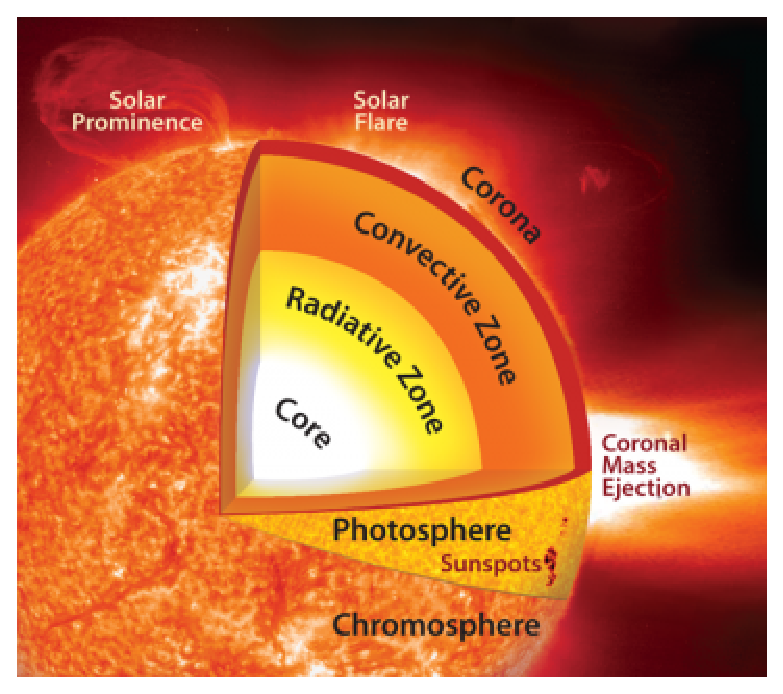
\includegraphics[width=0.9\textwidth]{new_figs/SolarStructure.eps}}
\end{center}
\column{0.55\textwidth}
\ \hskip 1cm \azul{Atmosphere}
\begin{itemize}
\item Photosphere (T $\approx 5.5$\, kK, $n \approx 10^{17}\ {\rm cm}^{-3}$)
\item Chromosphere (T $\approx 20$\, kK, $n \approx 10^{11}\ {\rm cm}^{-3}$)
\item Transition Region (Thickness 100 km)
\item Corona (T $\approx 1-10$\, MK, $n \approx 10^{10-7}\ {\rm cm}^{-3}$)
\end{itemize}
\begin{center}
{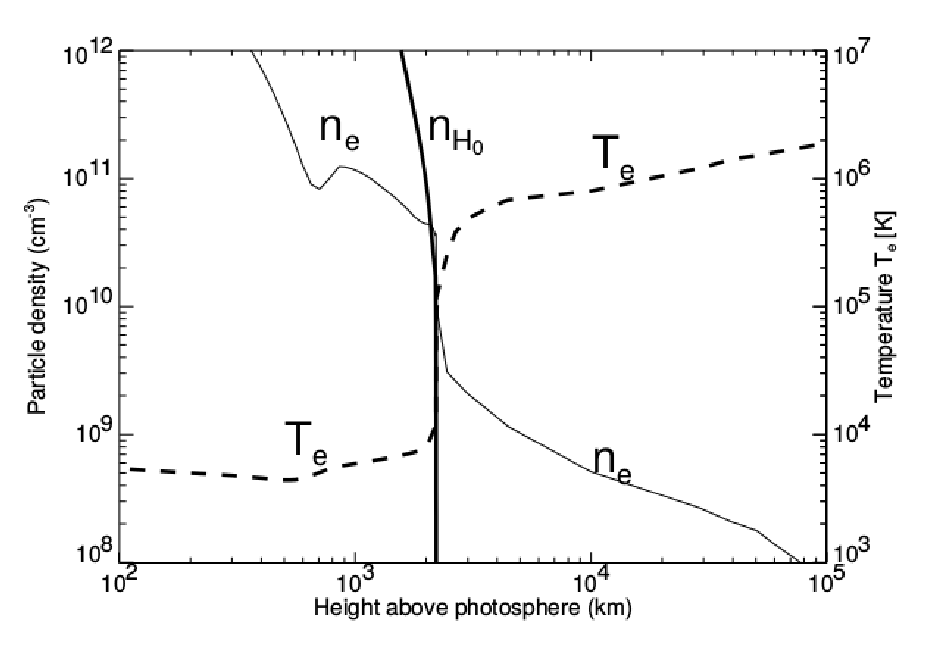
\includegraphics[width=0.675\textheight]{new_figs/region_transicion_fede.eps}}
\end{center}
\end{columns}
}
\end{comment}
%---------------------------------------------------------------------------
\frame{
\titulo{Corona Solar}
\footnotesize
\vspace{-0.25cm}
\begin{center}
{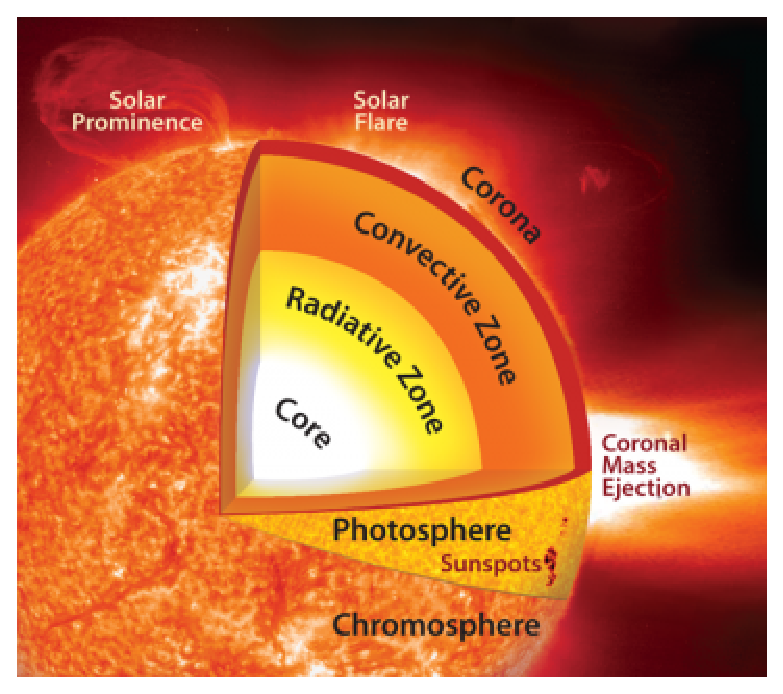
\includegraphics[width=0.35\textwidth]{new_figs/SolarStructure.eps}}
{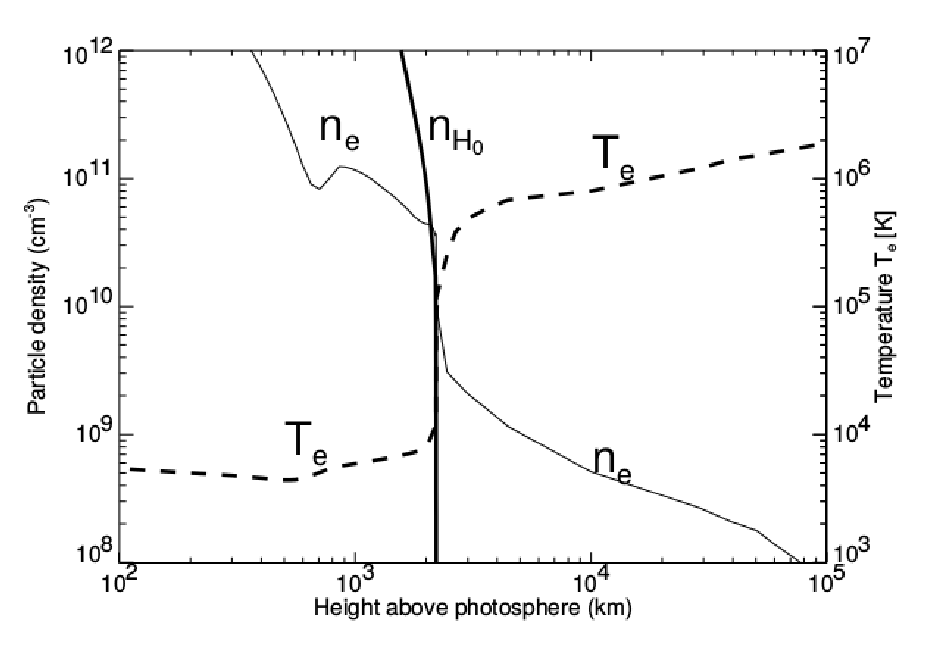
\includegraphics[width=0.5\textwidth]{new_figs/region_transicion_fede.eps}}
\end{center}
 Corona (T $\approx 1-10$\, MK, $n \approx 10^{10-7}\ {\rm cm}^{-3}$)
\begin{itemize}
 \vspace{0.5cm}
 \item La baja corona es ópticamente delgada y emite eficientemente en el rango EUV.\\
 %\item The corona is \azul{optically thin} in the UV, \azul{EUV}, X, \azul{WL} ranges.\\
%\item Images are thus 2D projections of the underlying 3D emitting structure.
% \salto
% \item El plasma emisor es governado por el \azul{campo magn\'etico coronal} congelado a la materia, para el cual {no se dispone de mediciones} (que son fotosf\'ericas).
 \mediosalto
%\item El avance de los modelos físicos necesitan información 3D coronal de parámetros fundamentales: $N_e$, $T_e$ y abundancias químicas.

%\item Las imágenes son proyecciones 2D de estructuras emisoras 3D.
%\item Advancement of physical models is in need of 3D information of the coronal fundamental parameters ${\bf B}, N_e, T_e$ and chemical abundances.
\end{itemize}

}
%-----------------------------
%\frame{ 
%\begin{columns}
%\column{0.8\textwidth}
%\begin{center}
%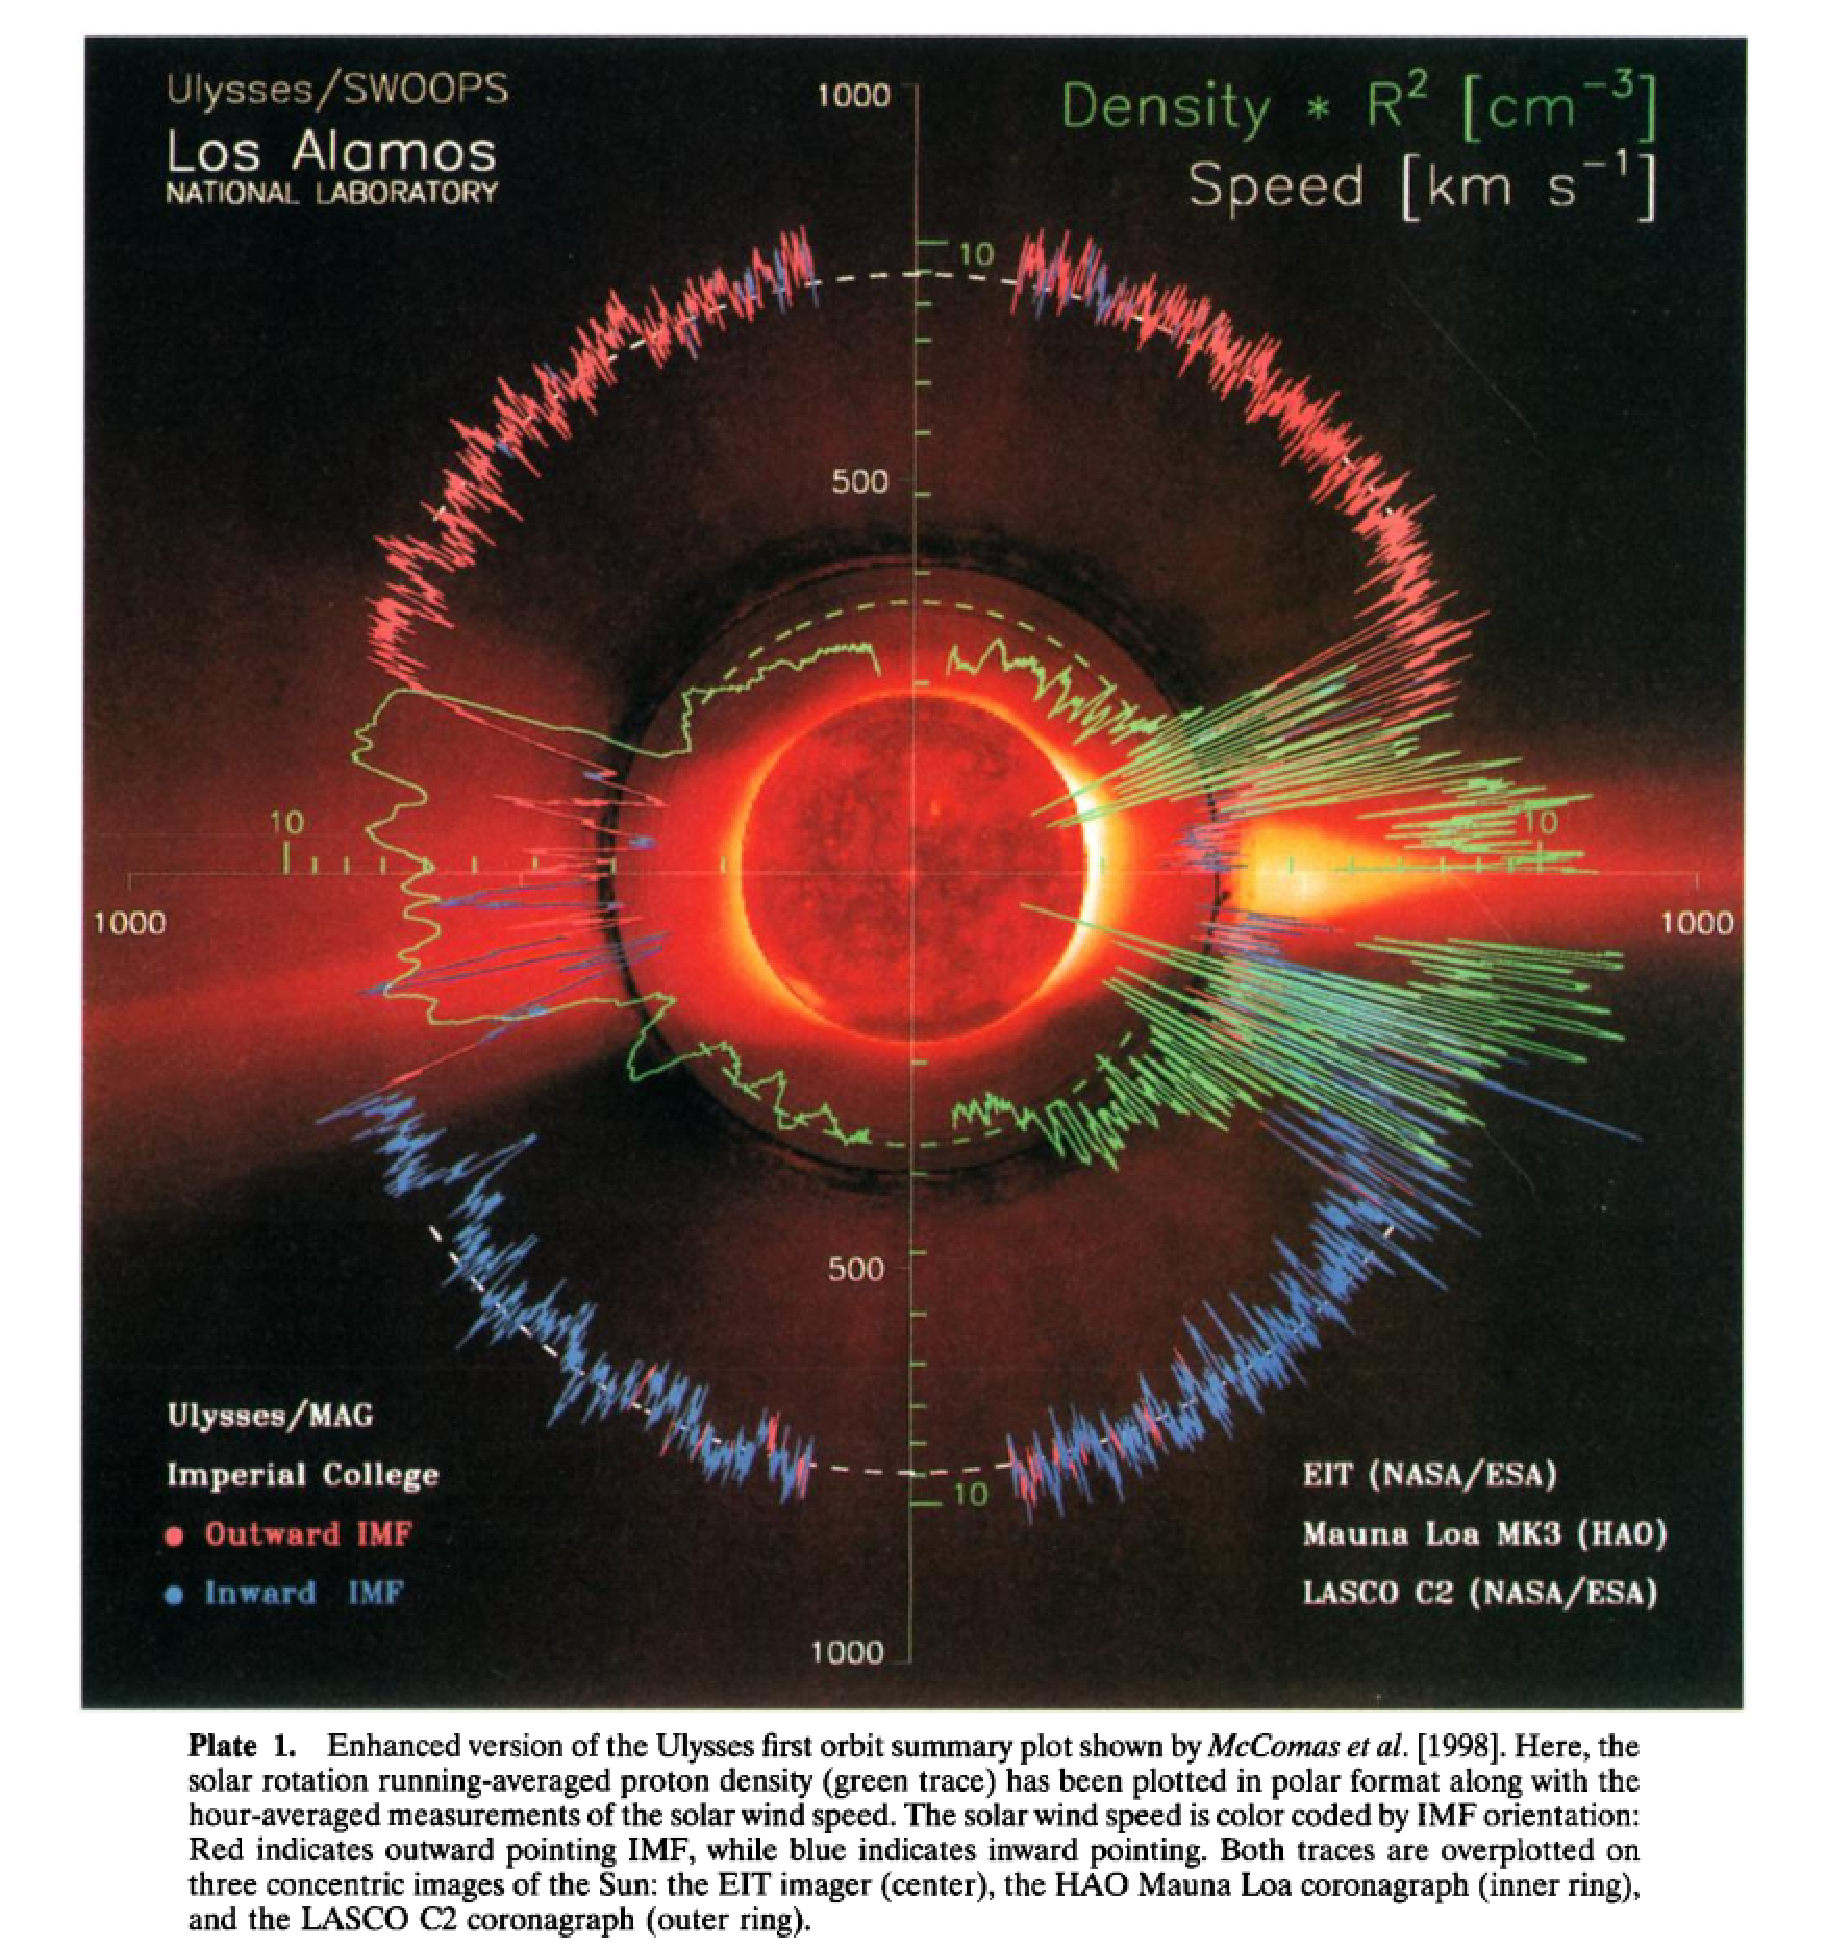
\includegraphics[width=0.99\textwidth]{new_figs/ulysses.pdf}
%\end{center}
%\column{0.2\textwidth}
%\begin{center}
%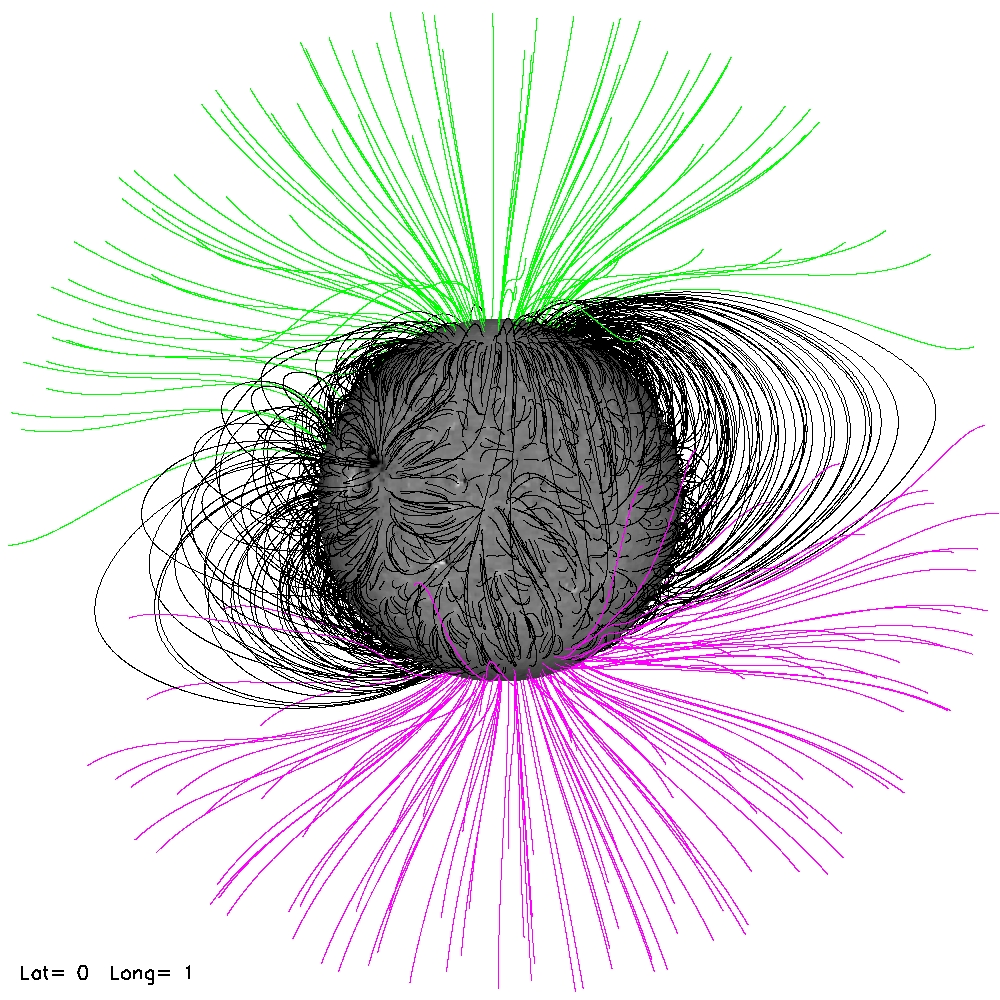
\includegraphics[width=0.99\textwidth]{new_figs/CR2223_PFSS_GONG_mrnqs_275.jpg}
%\end{center}
%\end{columns}
%}

\frame{
\footnotesize
\vskip -0.3cm
\begin{columns}
\column{0.7\textwidth}
\begin{center}
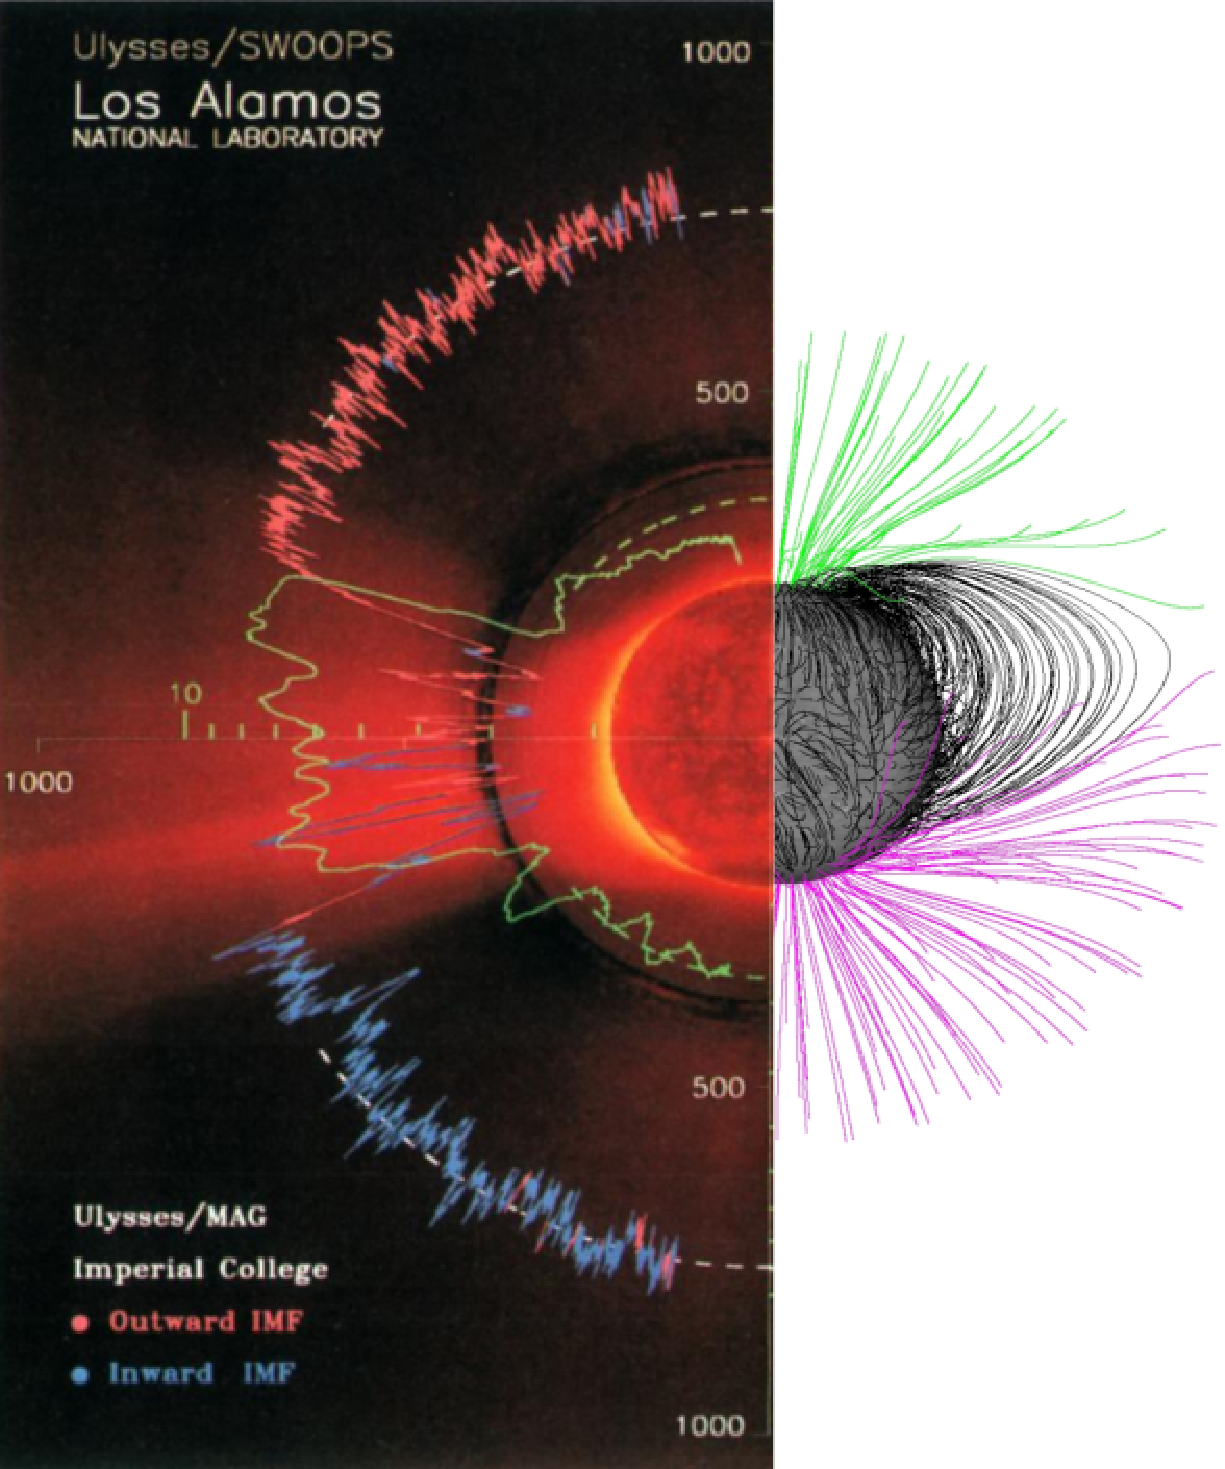
\includegraphics[width=0.9\textwidth]{new_figs/mezcla_pfss_ulysses.pdf}
\end{center}
\column{0.3\textwidth}
%\vskip -0.3cm
\begin{itemize}
  \item El plasma fluye por las líneas abiertas
  \vskip 0.3cm
  \item Líneas abiertas de alta latitud presentan régimen rápido y de baja densidad.
  \vskip 0.3cm
  \item Líneas abiertas de baja latitud presentan régimen lento y de alta densidad.
\end{itemize}
 \vskip 1.5cm

 \tiny McComas et al. 2000 \\
 (\jgr)\\
 \vskip 0.5cm
\tiny Suess et al. 2009 \\
(\jgr)\\
\end{columns}
}
%------------------------------
\frame{
\titulo{Tomografía Solar Rotacional (TSR)}
\footnotesize
\vspace{-0.2cm}
\begin{center}
%The corona is \azul{optically thin} in the UV, \azul{EUV}, X, \azul{WL} ranges.\\
%By inverting for the \azul{3D EUV emissivity from time series of images} it allows inferring the 3D $N_e$ and $T_e$ of the global corona.
%The object of study is the solar corona.\\
%The solar rotation provides the necessary 360\deg view angles.
El objeto de estudio es la Corona Solar.\\
\end{center}
%\vspace{-1.5cm}
%\begin{columns}
%\vspace{-1cm}
%\column{0.6\textwidth}
\begin{itemize}
\item \azul{Corona-E:} Emisión de iones coronales en UV, \azul{EUV} y X.
\item \azul{TSR-EUV} $\rightarrow$ emisividad EUV 3D  $\rightarrow$ DEM 3D $\rightarrow$$N_e$ y $T_e$ 3D
\item 1$^{\rm er}$ TSR-EUV:\\ 
Frazin, Vásquez \& Kamalabadi (ApJ 2009)\\
Vásquez, Frazin \& Kamalabadi (SolPhys 2009)
\end{itemize}
%\column{0.4\textwidth}
%\vskip 1.2cm
%\begin{center}
%\azul{White Light}
%\includegraphics[height=0.7\textwidth]{new_figs/20171215_175739_kcor_l15_extavg.eps}
%\includegraphics[height=0.6\textwidth]{new_figs/LASCOC2_comet.eps}
%\mediosalto
%\azul{EUV} \\
%\includegraphics[height=0.6\textwidth]{new_figs/2017_12_15_19_11_15_AIA_171.png}
%\includegraphics[height=0.3\textwidth]{new_figs/2017_12_15_19_11_15_AIA_193.png}
%\includegraphics[height=0.3\textwidth]{new_figs/2017_12_15_19_11_15_AIA_211.png}
%\end{center}
%\end{columns}
\begin{center}
La rotación solar provee los diferentes ángulos de visión necesarios.
\end{center}
\begin{columns}
%\column{0.1\textwidth}
%\vskip 1cm
%195 \AA\\
%1.5 MK

\column{0.23\textwidth}
\begin{center}
Long = 360\deg\\
\framebox{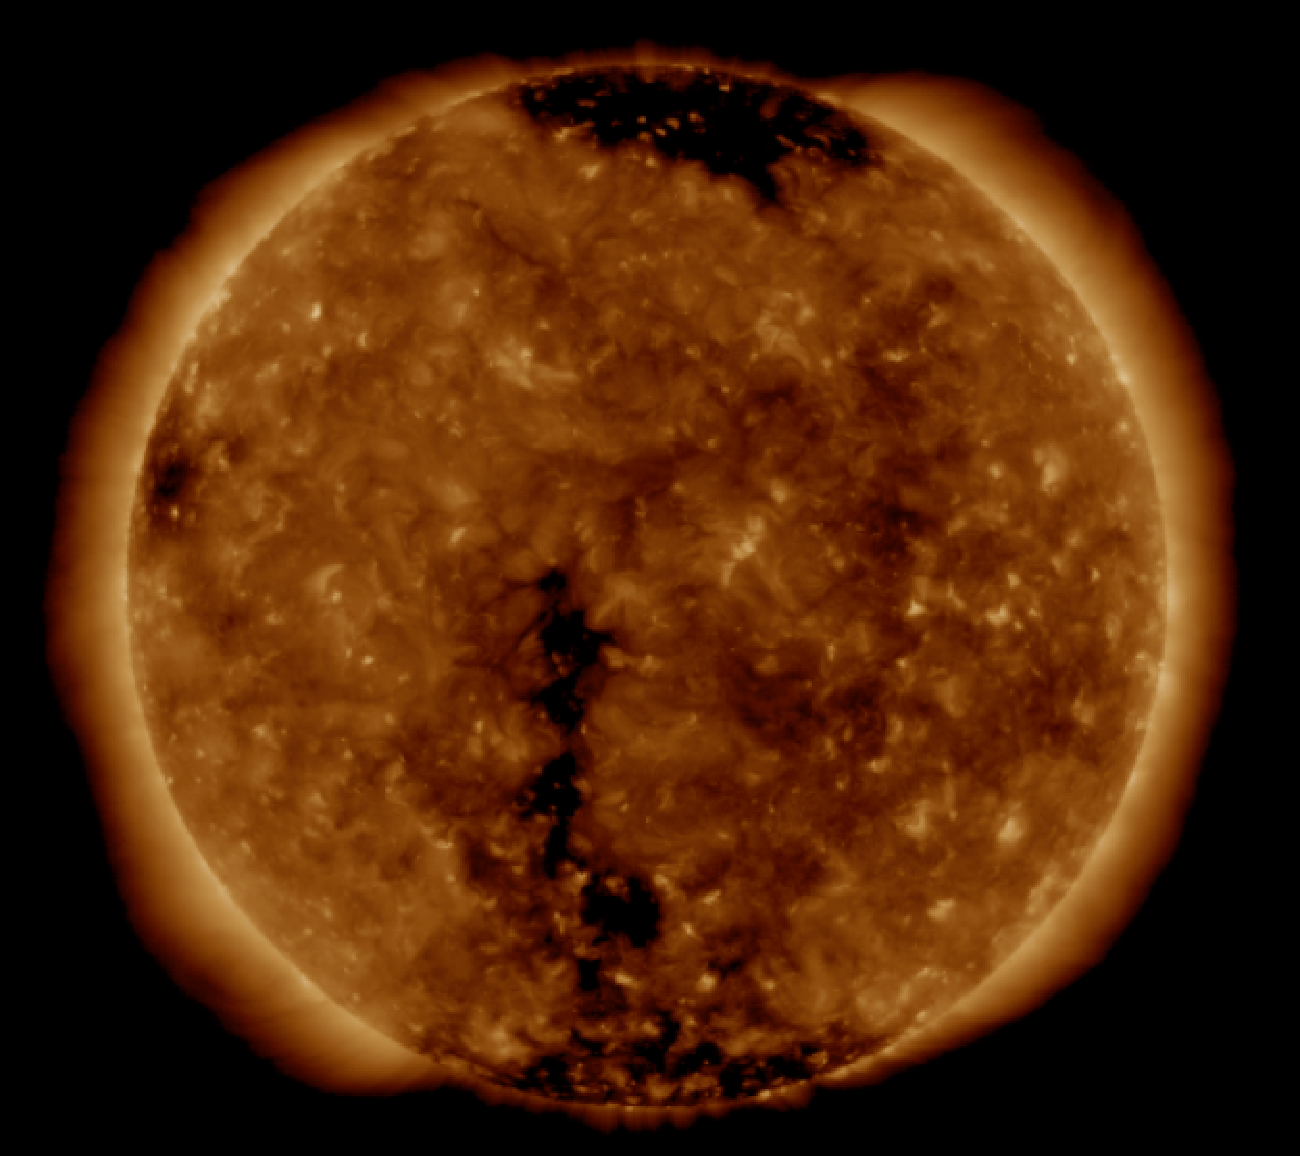
\includegraphics[width=\linewidth]
{new_figs/banda193_1.pdf}}
\end{center}
\column{0.23\textwidth}
\begin{center}
Long = 270\deg\\
\framebox{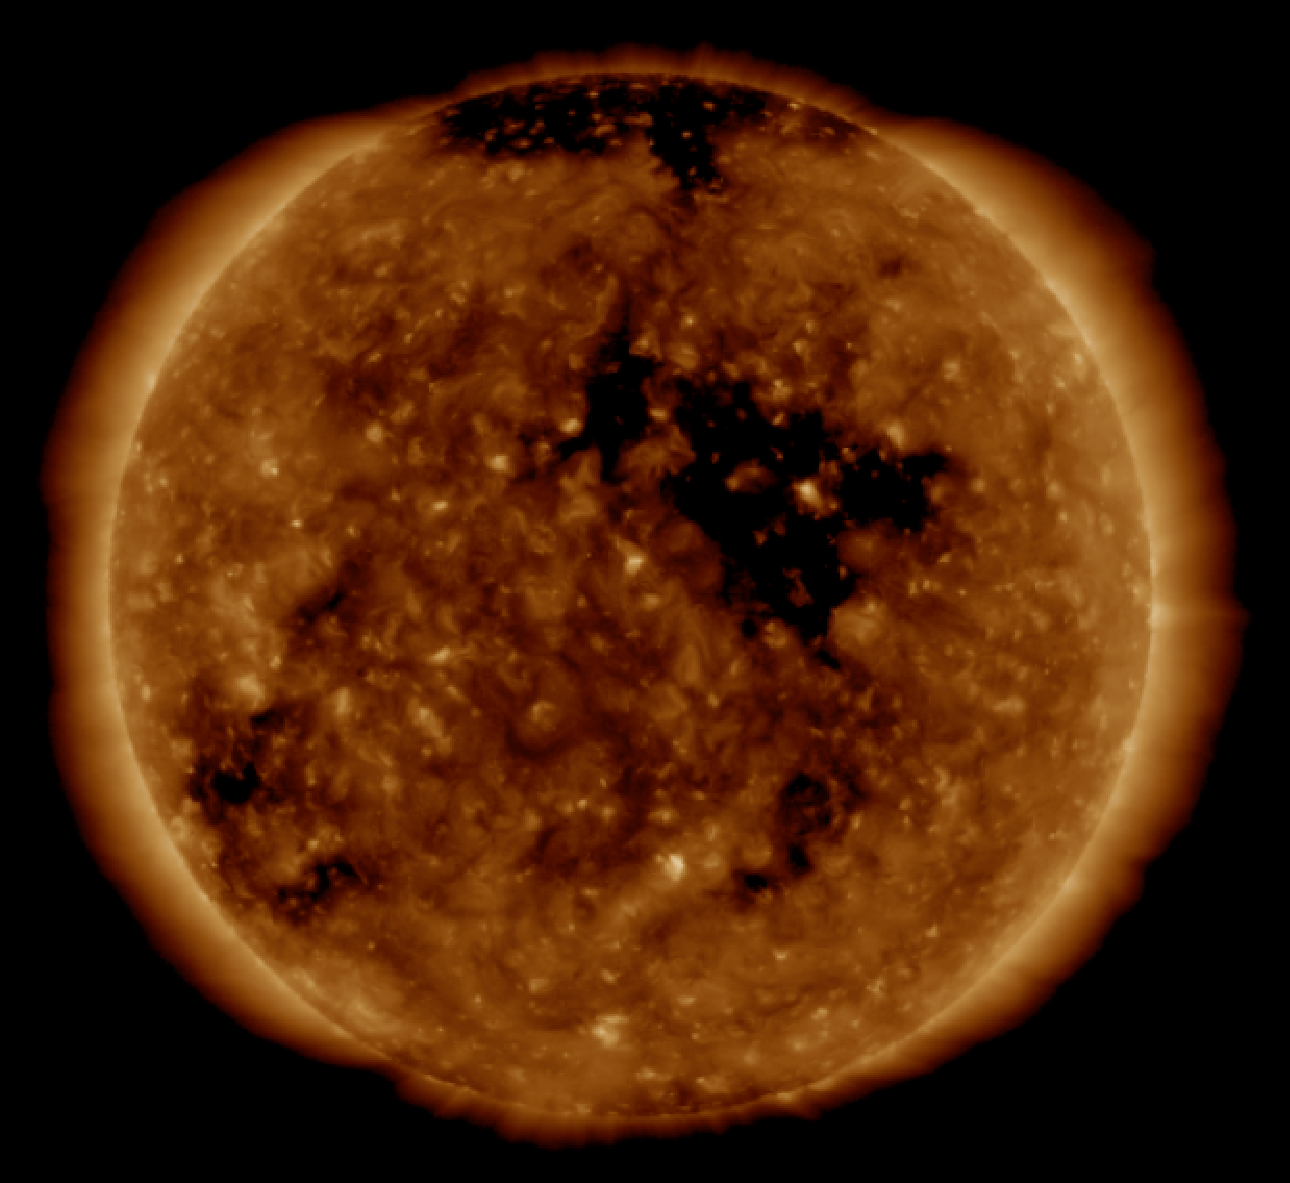
\includegraphics[width=\linewidth]
{new_figs/banda193_2.pdf}}
\end{center}
\column{0.23\textwidth}
\begin{center}
Long = 180\deg\\
\framebox{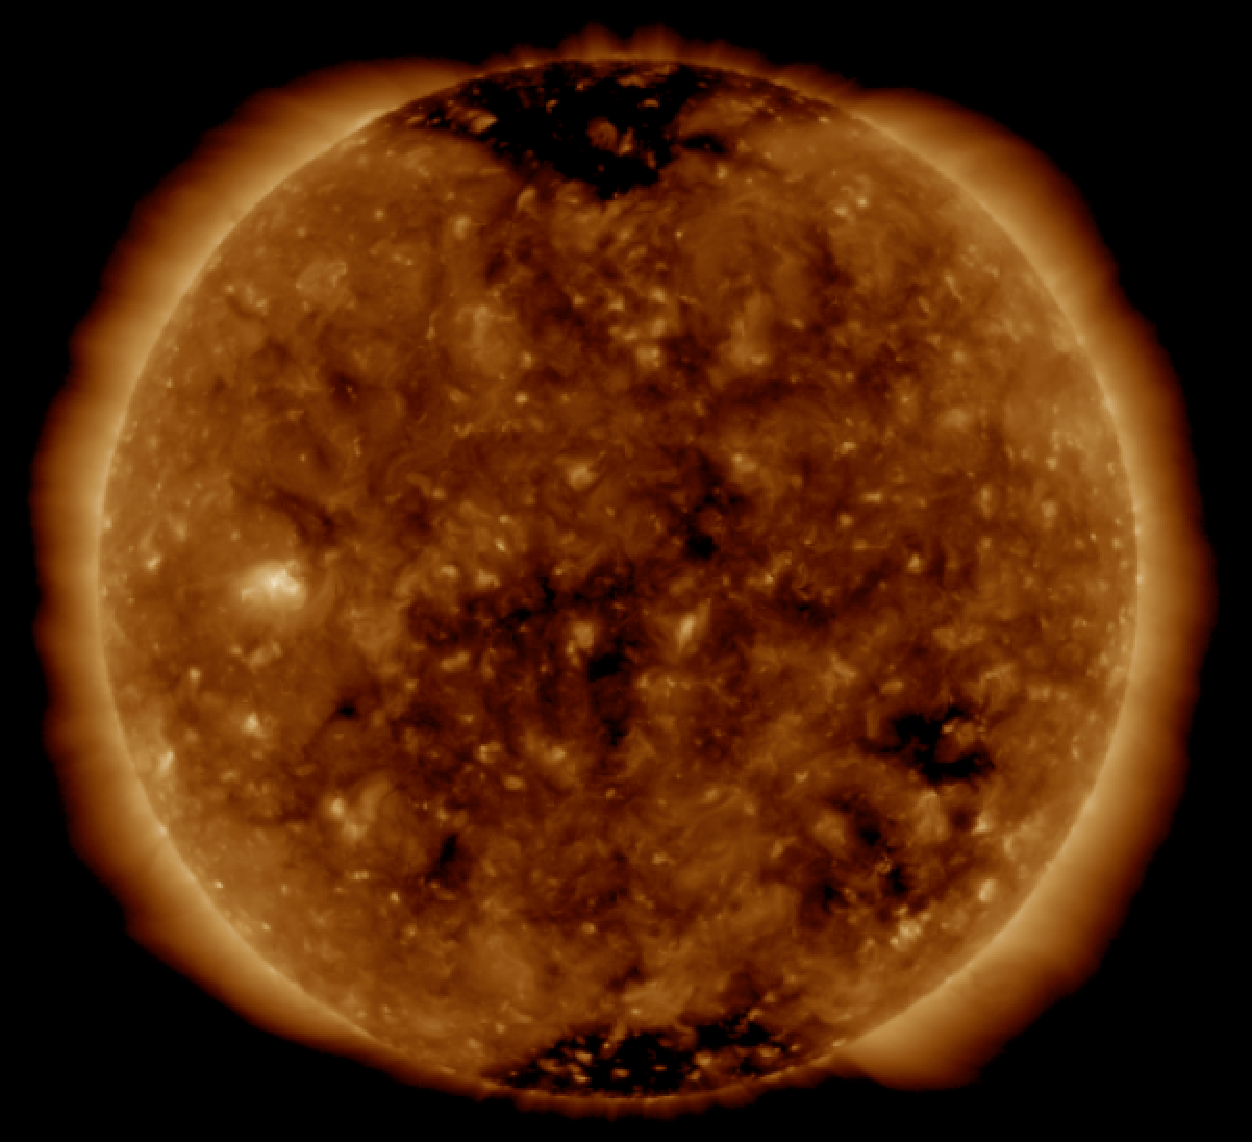
\includegraphics[width=\linewidth]
{new_figs/banda193_3.pdf}}
\end{center}
\column{0.23\textwidth}
\begin{center}
Long = 90\deg\\
\framebox{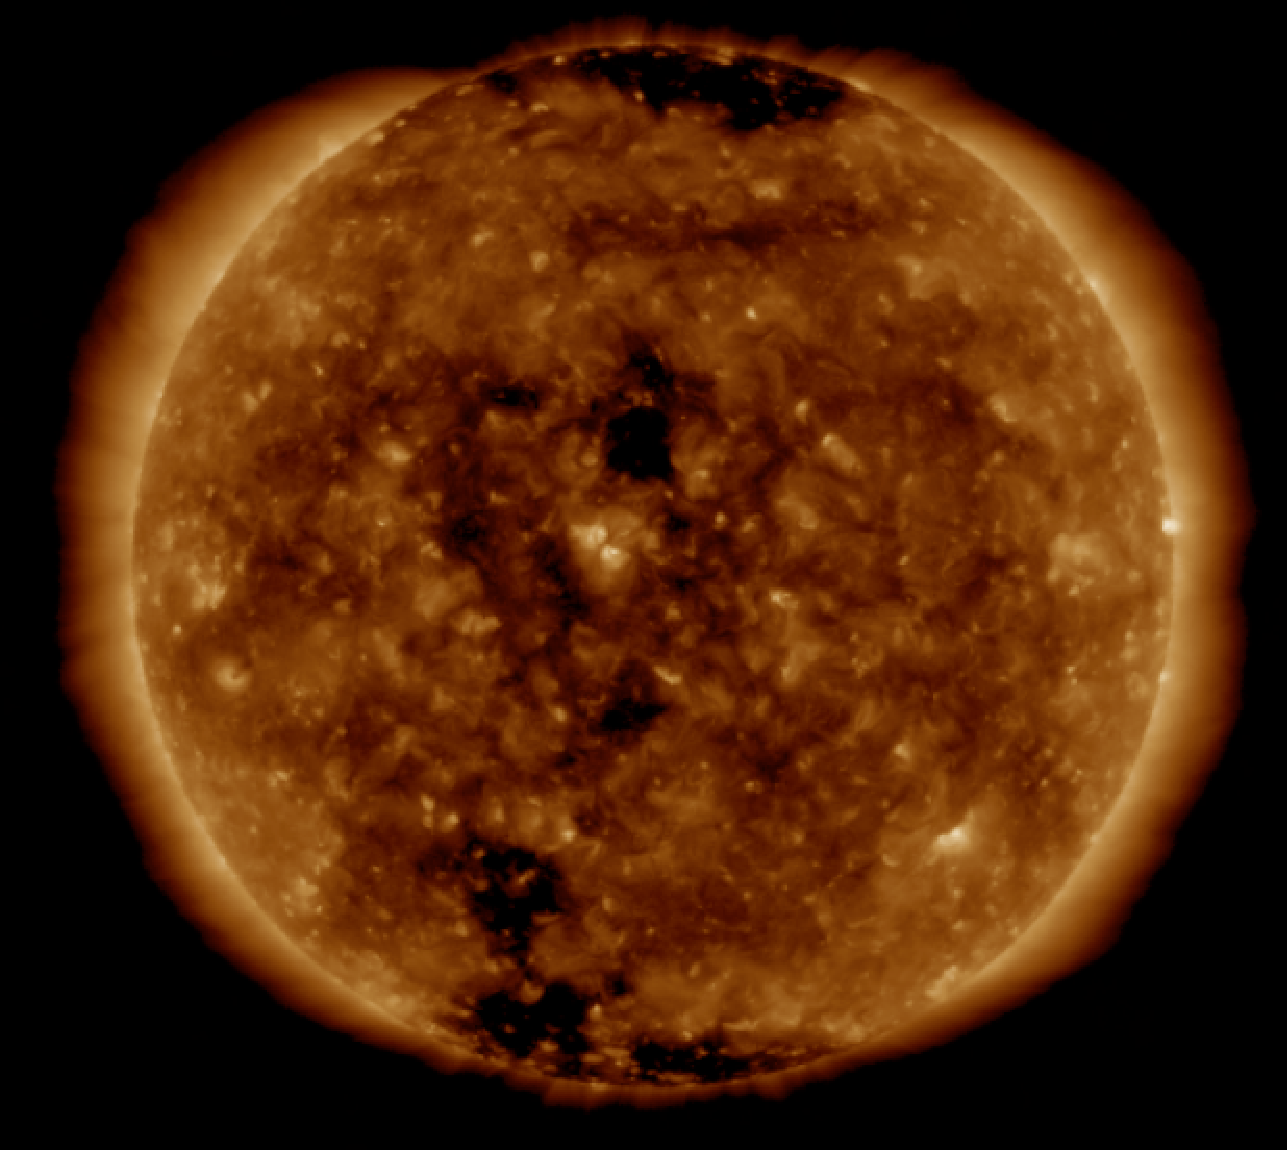
\includegraphics[width=\linewidth]
{new_figs/banda193_4.pdf}}
\end{center}
\end{columns}
}

%-----------------------------------
\begin{comment}
\frame{ 
\vspace{-0.35cm}
\begin{columns}
\noindent
\column{0.075\textwidth}
\vskip 0.8cm
{\footnotesize
\ 171 \AA
\vskip 1.75cm
\ 195 \AA
\vskip 1.65cm
\ 284 \AA
}
\column{\textwidth}
\begin{center}
{\footnotesize
\ \ Data Images \hfill $\rightarrow$ \hfill 3D Band Emissivity \hfill $\rightarrow$ \hfill Synthetic Images\ \ \ \
}\\
\framebox{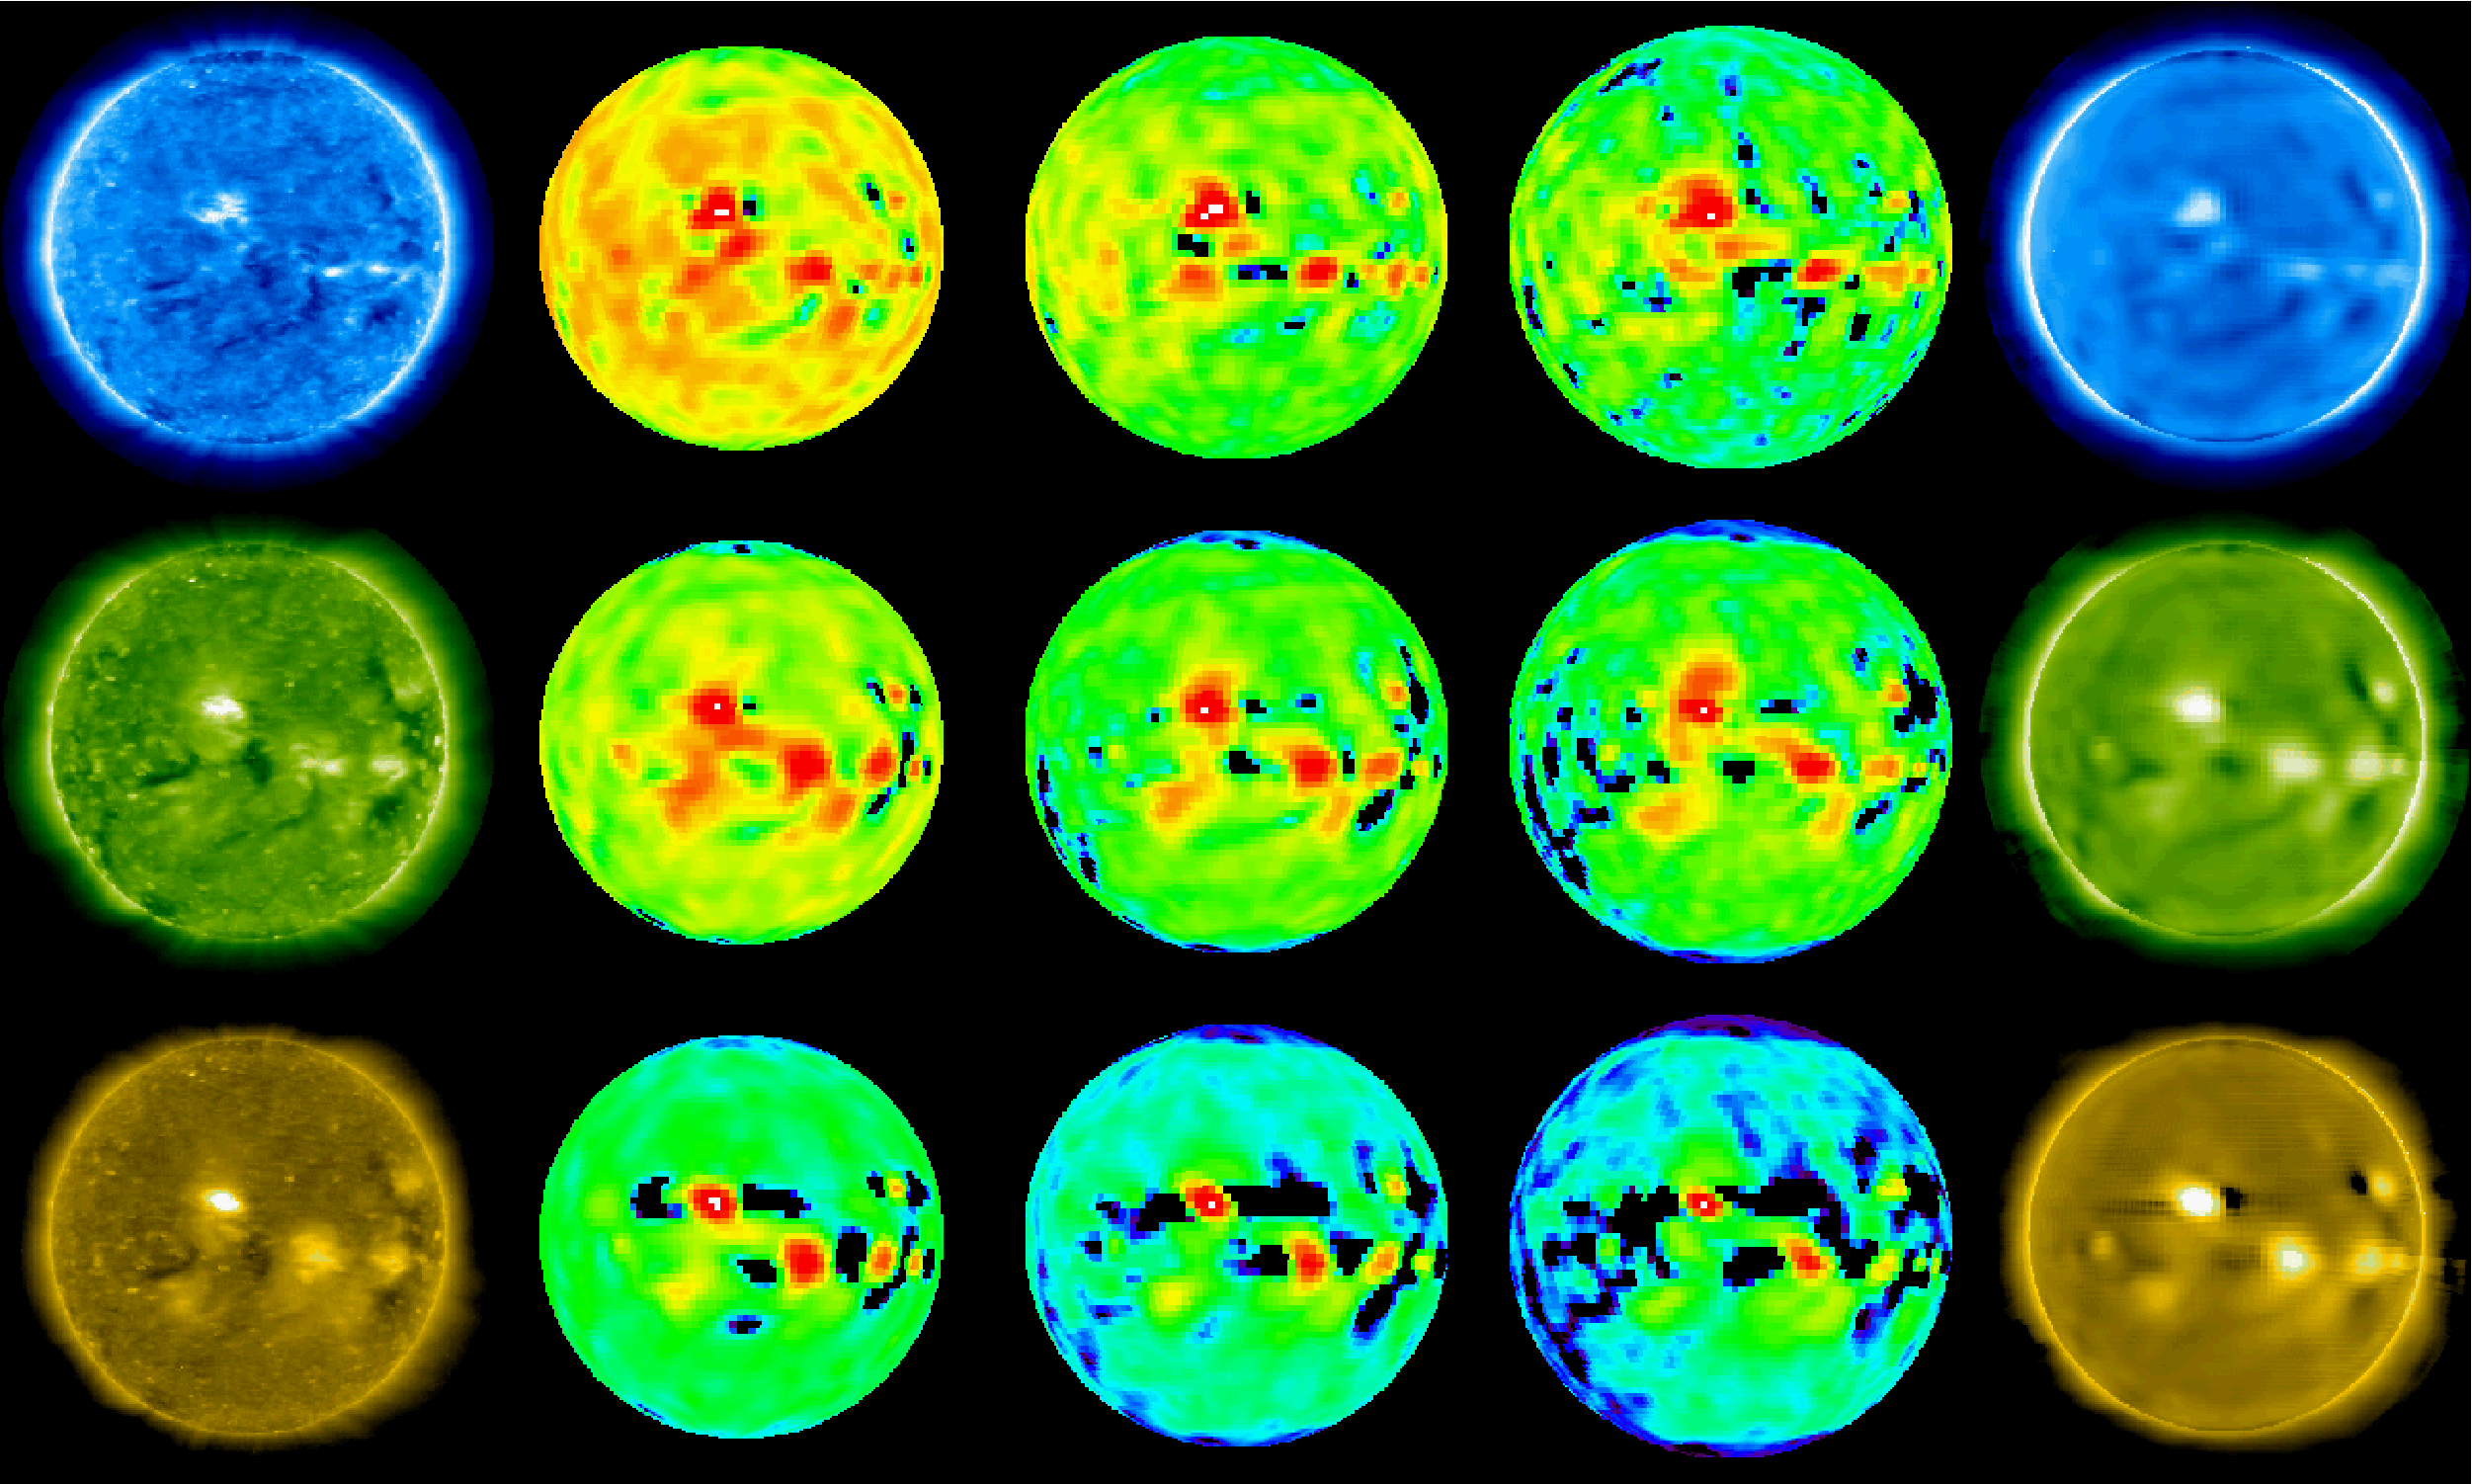
\includegraphics[width=0.95\linewidth]{new_figs/frame_050_test.pdf}}\\
\footnotesize
 1.035 $\mrsun$ \hskip 1cm 1.085 $\mrsun$ \hskip 1cm 1.135 $\mrsun$ \hfil
\end{center}
\end{columns}
%\begin{columns}
% \column{0.4\textwidth}
 
%\azul{I_{k,j}} = \azul{
%\int_{\mathrm{LOS}} \mathrm{d}l} \ 
%\rojo{FBE_k \left(\azul{\br_j(l)}\right)}

$\azul{I_\mathrm{b}} = \azul{
\int_{\mathrm{LDV}} \mathrm{d}l} \ 
\rojo{E_{b}}$

 \hfill Vásquez et al. (2016)
% \column{0.6\textwidth}
%\end{columns}
}
\end{comment}
%-------------------------------
\frame{
\titulo{Temperaturas características de la Corona Solar}
\footnotesize
\begin{center}
%EIT/SOHO y EUVI/STEREO \azul{3 bands:} \azul{0.5-2.75 MK}\\
{AIA/SDO} \azul{4 bandas:} \azul{0.5-4.0 MK}\\
\begin{figure}[ht]
\figu{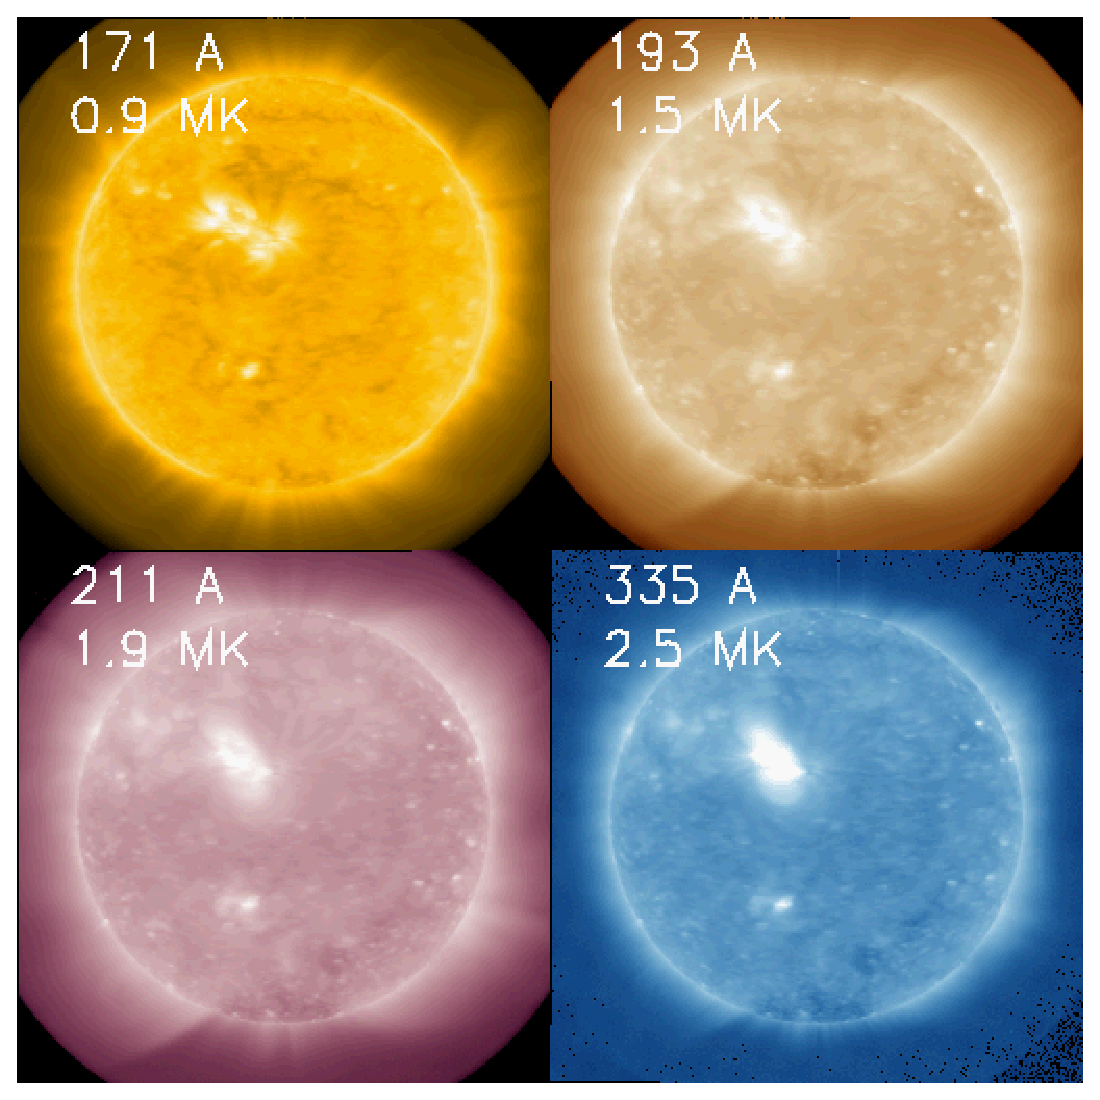
\includegraphics[height=0.375\linewidth]{new_figs/panel.eps}}
\figu{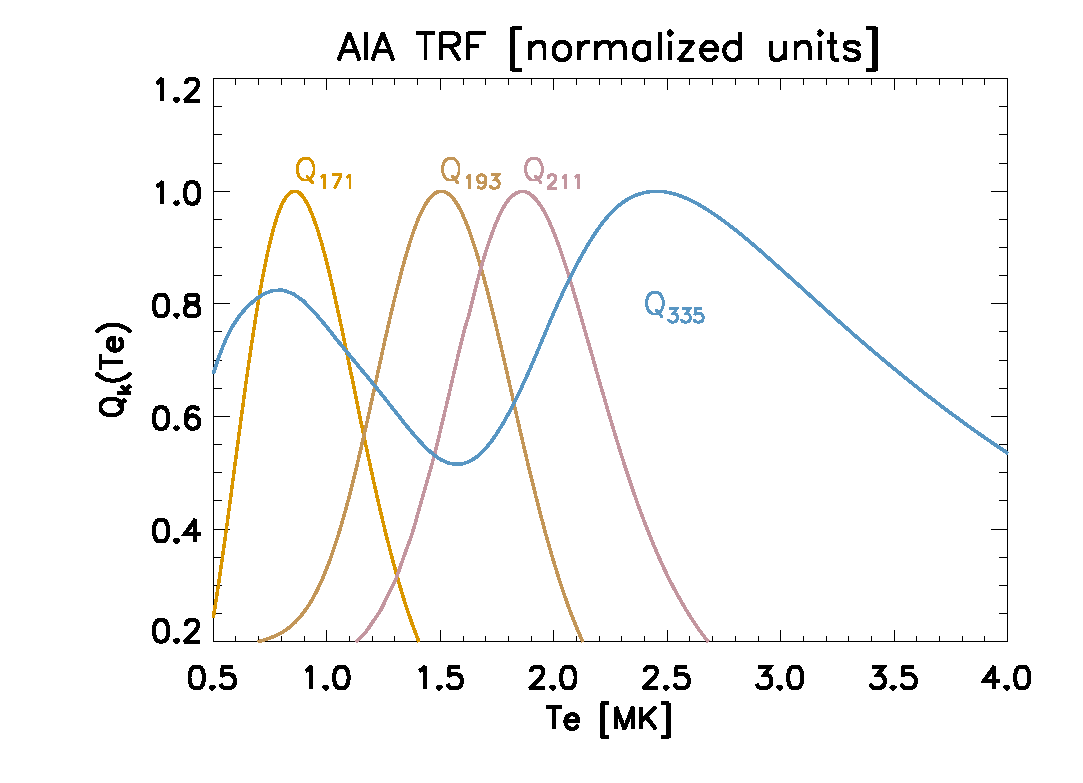
\includegraphics[height=0.375\linewidth]{new_figs/qkl.eps}}
\end{figure}
\end{center}
%\tiny
% \hfill Vásquez et al. (2016) \\
\begin{itemize}
\item $\azul{I_\mathrm{b}} = \azul{\int_{\mathrm{LDV}} \mathrm{d}l} \ \rojo{E_{b}}$ \hfill
\item  $\azul{E_{b} }  =  \azul{\int \mathrm{d}T \  R_b(T)  \rojo{{\sf LDEM}(T)} }$ $\rightarrow$
$\left< N_e^2\right> = \int \mathrm{d} T \ \, \rojo{{\sf LDEM}(T)}$\\
\qquad \qquad \qquad \qquad \qquad \qquad \ \ $\rightarrow$ $T_{m}   = \frac{1}{\left< N_e^2\right> } \int \mathrm{d}T\ T \ \, \rojo{{\sf LDEM}(T)}$\\
\end{itemize}
\hfill (Nuevo et al. 2015, ApJ)
}

%---------------------------------
\frame{ 
\vspace{-0.05cm}
\titulo{Mapas de carrington tomográficos}
\footnotesize

\begin{center}
%  Mínimo solar 2009 - Extreme UltraViolet Imager\\
{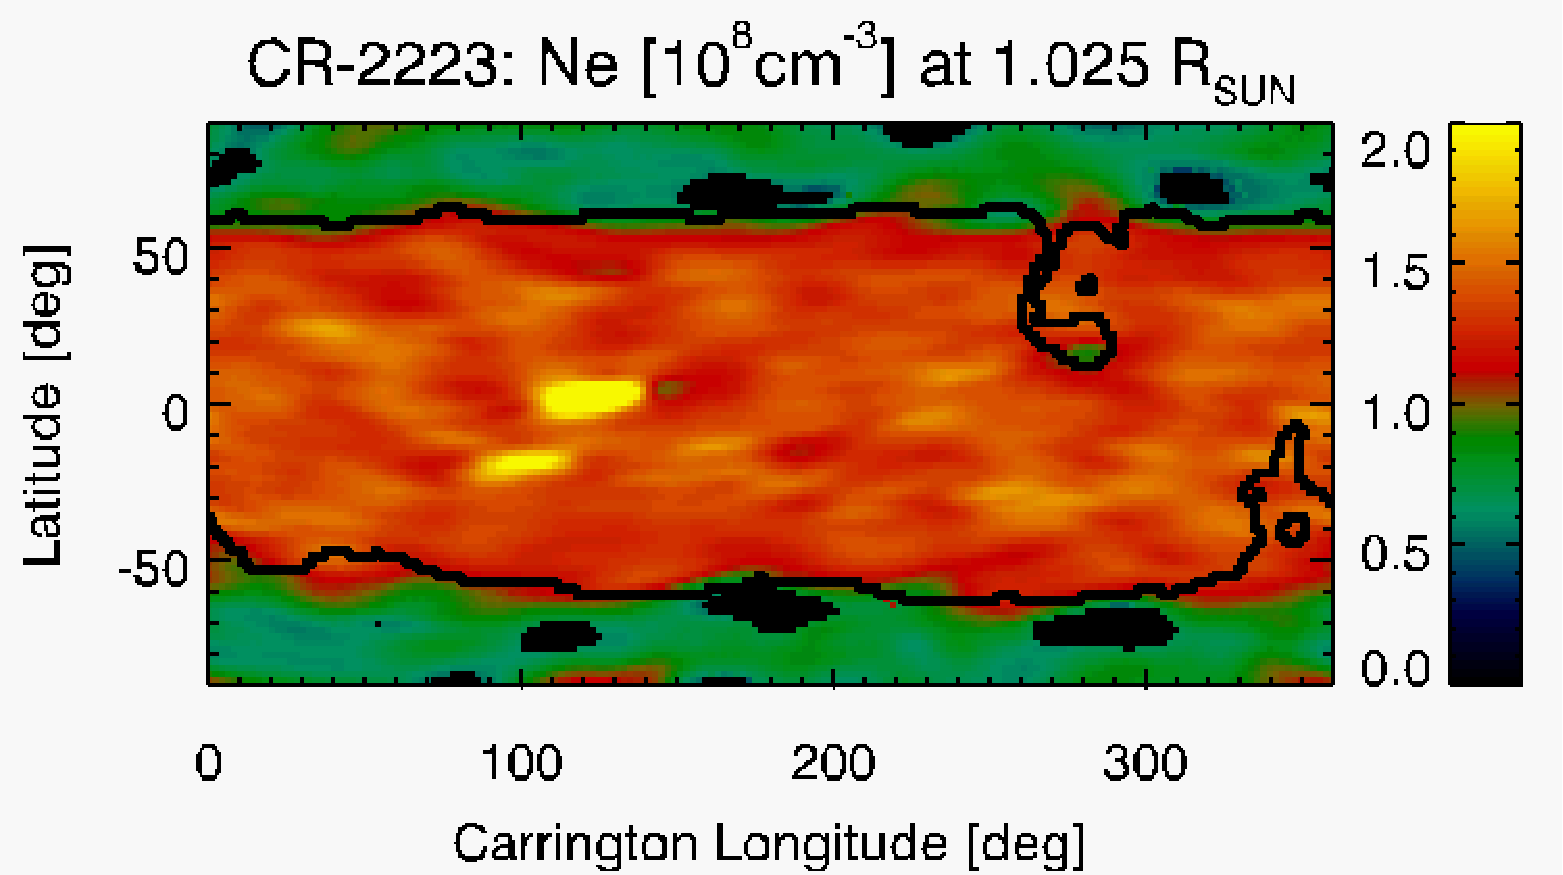
\includegraphics[width=0.6\textwidth]{new_figs/map_Ne_CR2223_DEMT-AIA_H1_L733_r3d_multistart_1025_Rsun_mapoc_awsom.pdf}}
%{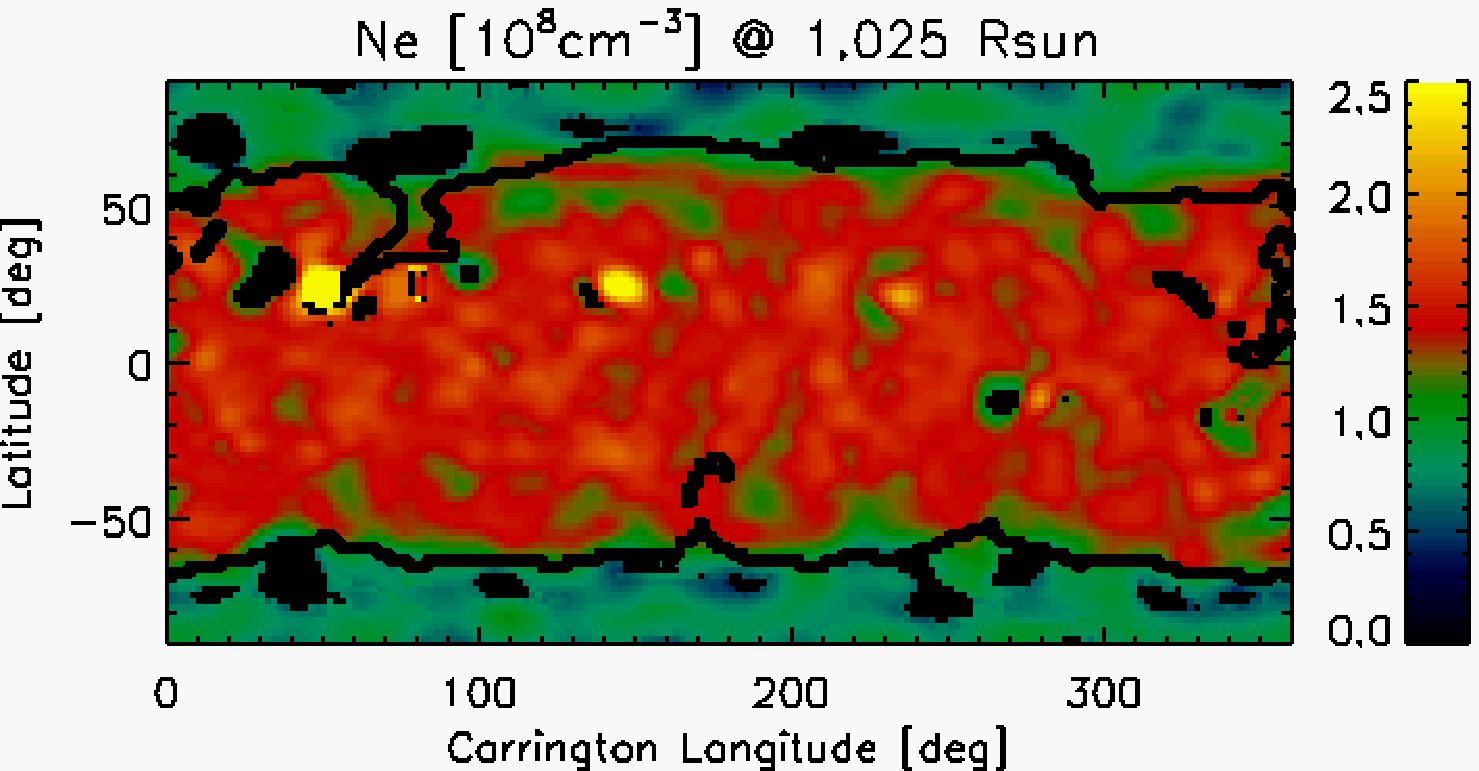
\includegraphics[width=0.46\textwidth]{new_figs/Ne_1025_CR2081.pdf}}
{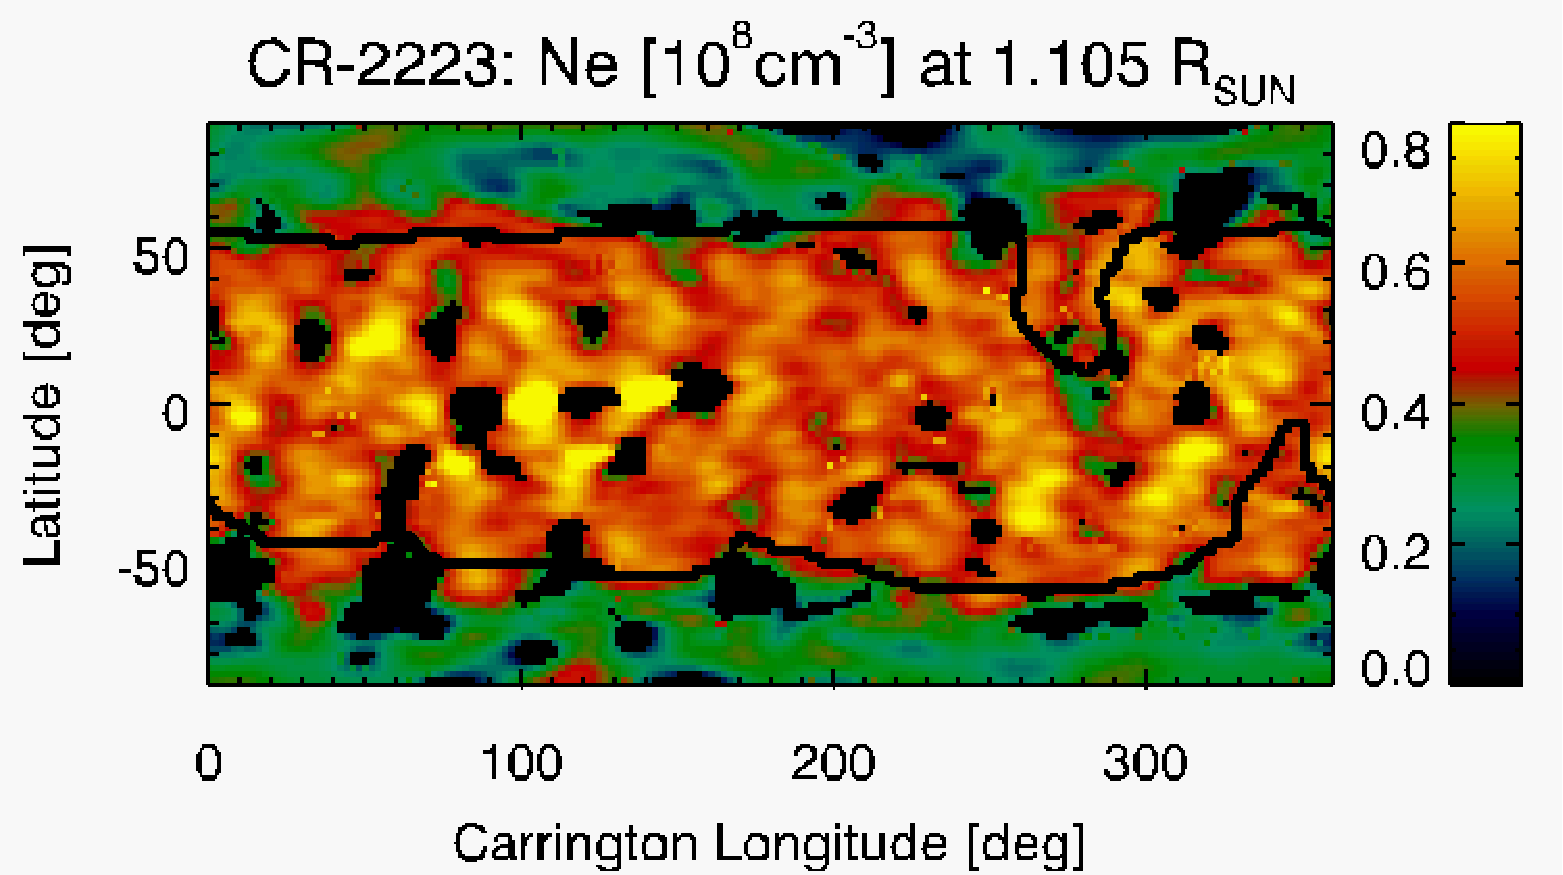
\includegraphics[width=0.6\textwidth]{new_figs/map_Ne_CR2223_DEMT-AIA_H1_L733_r3d_multistart_1105_Rsun_mapoc_awsom.pdf}}\\
%{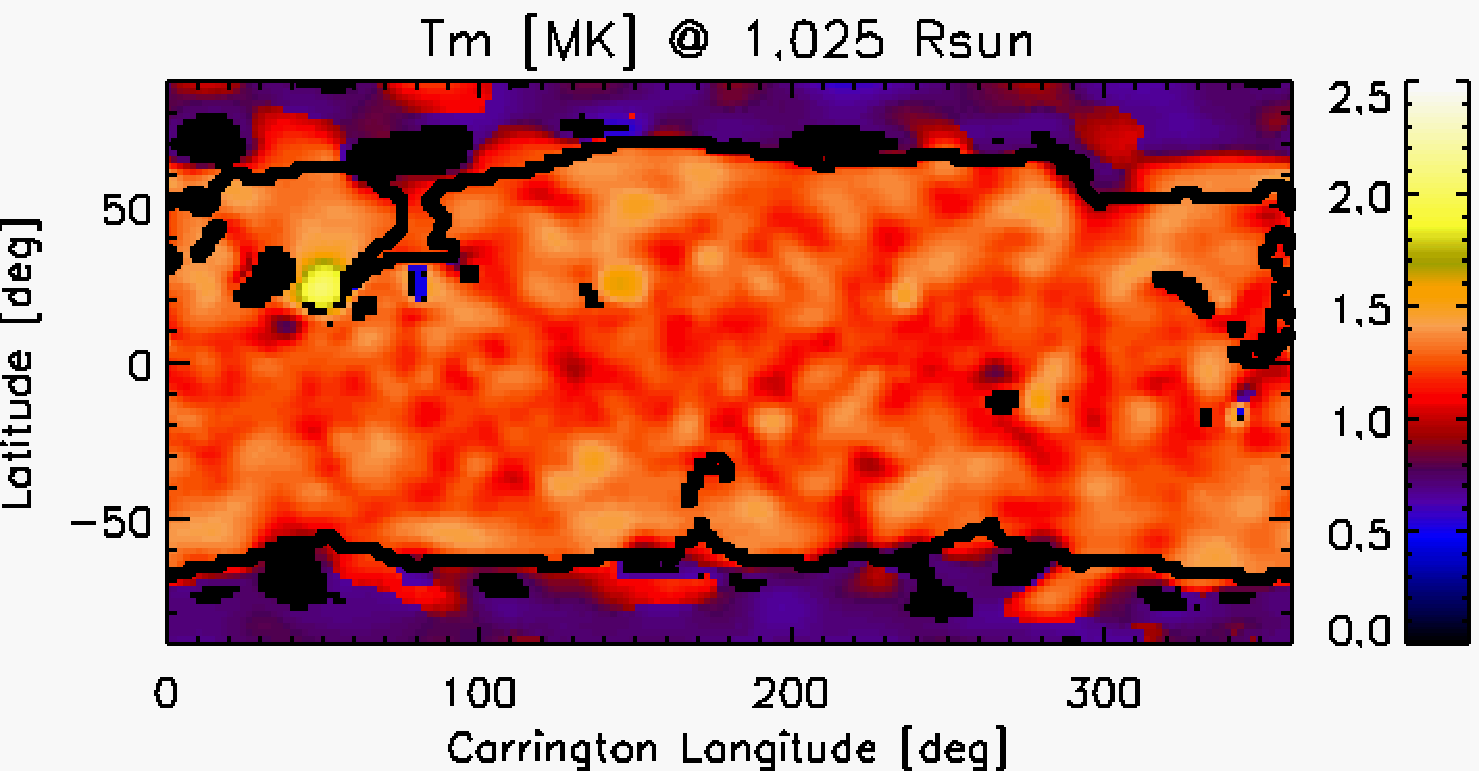
\includegraphics[width=0.46\textwidth]{new_figs/Tm_1025_CR2081.pdf}}\\
\end{center}
%(Lloveras et al. 2017, Solar Physics) $\rightarrow$ Incertezas sistemáticas en DEMT $\sim 10 \%$ \\
%Nuevo et al. 2013, APJ
}
%----------------------------------
\frame{
%\titulo{Validación del modelo AWSoM (SWMF)}
%\begin{itemize}
%  \item Vásquez et al 2008, APJ
%  \item Van del Holst 2010, APJ (Stereo, ACE)
%  \item Jin et al. 2012, APJ (ACE, Stereo, Lasco C2)
%  \item Whole Heliosphere Interval, 2012 (mínimo 2009)  
%  \item Oran et al. 2015, APJ (Ulysses, perfiles latitudinales con demt)
%  \item Colage XI (2018) presentamos una comparación del mínimo del 2009 y guiamos la validación de la baja corona.
%  \item Sachdeva et al. 2019, APJ. (AIA, Lasco C2, IPS, OMNI)
%\end{itemize}

\titulo{Modelo MHD-3D AWSoM}
\begin{itemize}
  \item MHD-3D: Alfvén Wave Solar Model (AWSoM), forma parte del Space Weather Modeling Framework (SWMF)
\item Calentamiento coronal dado por disipasión ondas de Alfvén \\(van der Holst et al.,  2014)
\item Abarca desde la cromosfera hasta 1 UA
\item Magnetograma sinóptico como condición de contorno (ADAPT-GONG)
\end{itemize}

\begin{columns}
\column{0.6\textwidth}
\begin{center}
%Magnetograma
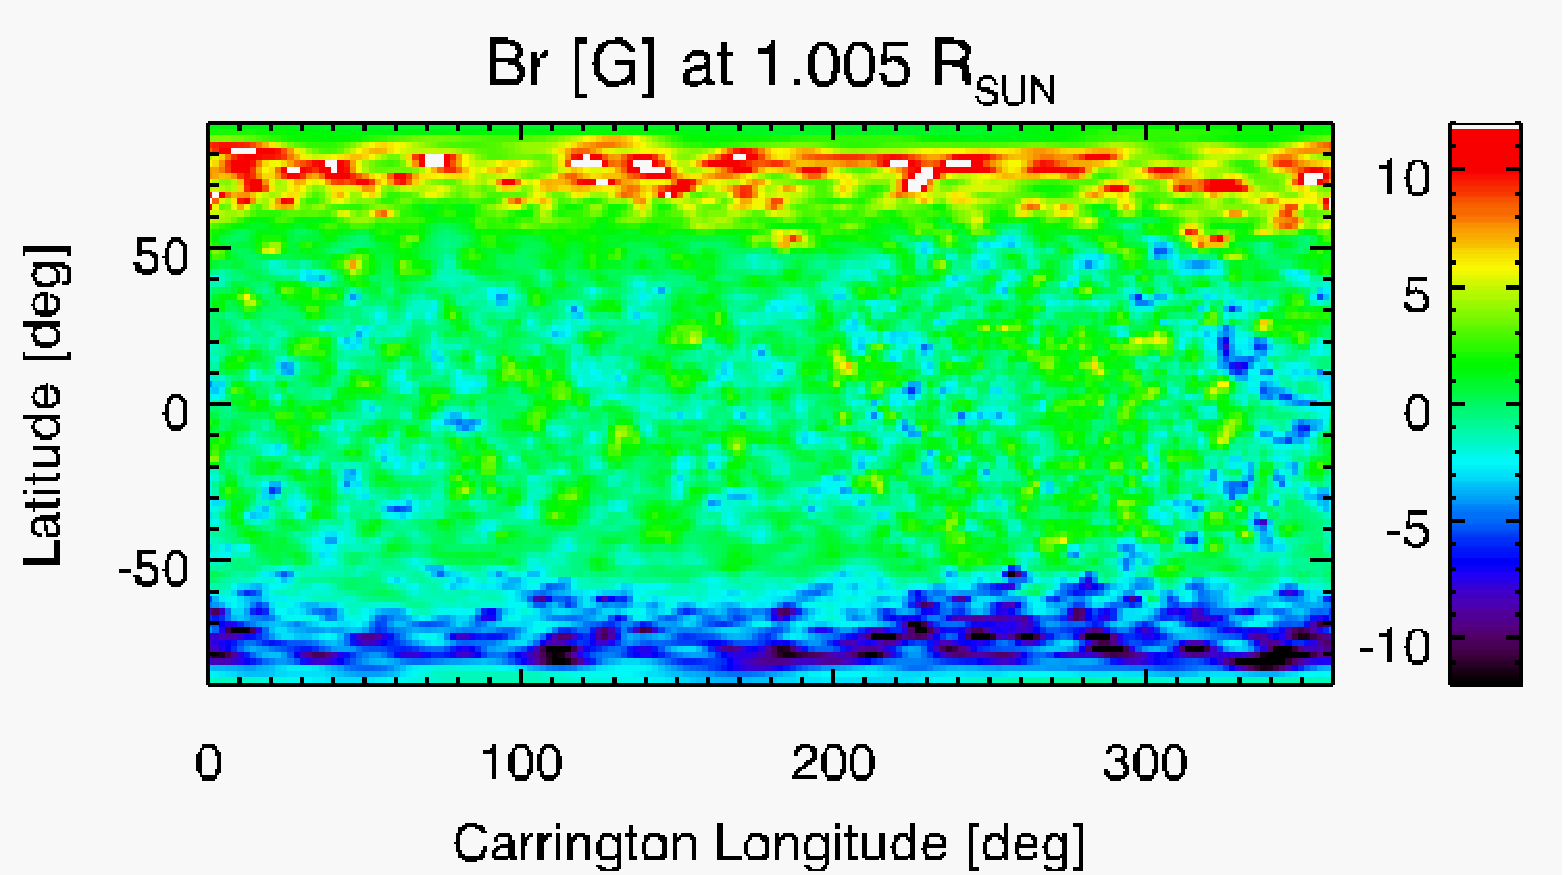
\includegraphics[width=0.99\textwidth]{new_figs/map_Br_awsom_2223_realization10_extended_new_1005_Rsun.pdf}
\end{center}
\column{0.4\textwidth}

Sachdeva et al. 2019, Apj.\\
Lloveras et al. 2020, SolPhys.\\
\end{columns}
}


%-----------------------------------
\frame{
%\titulo{}
\begin{center}
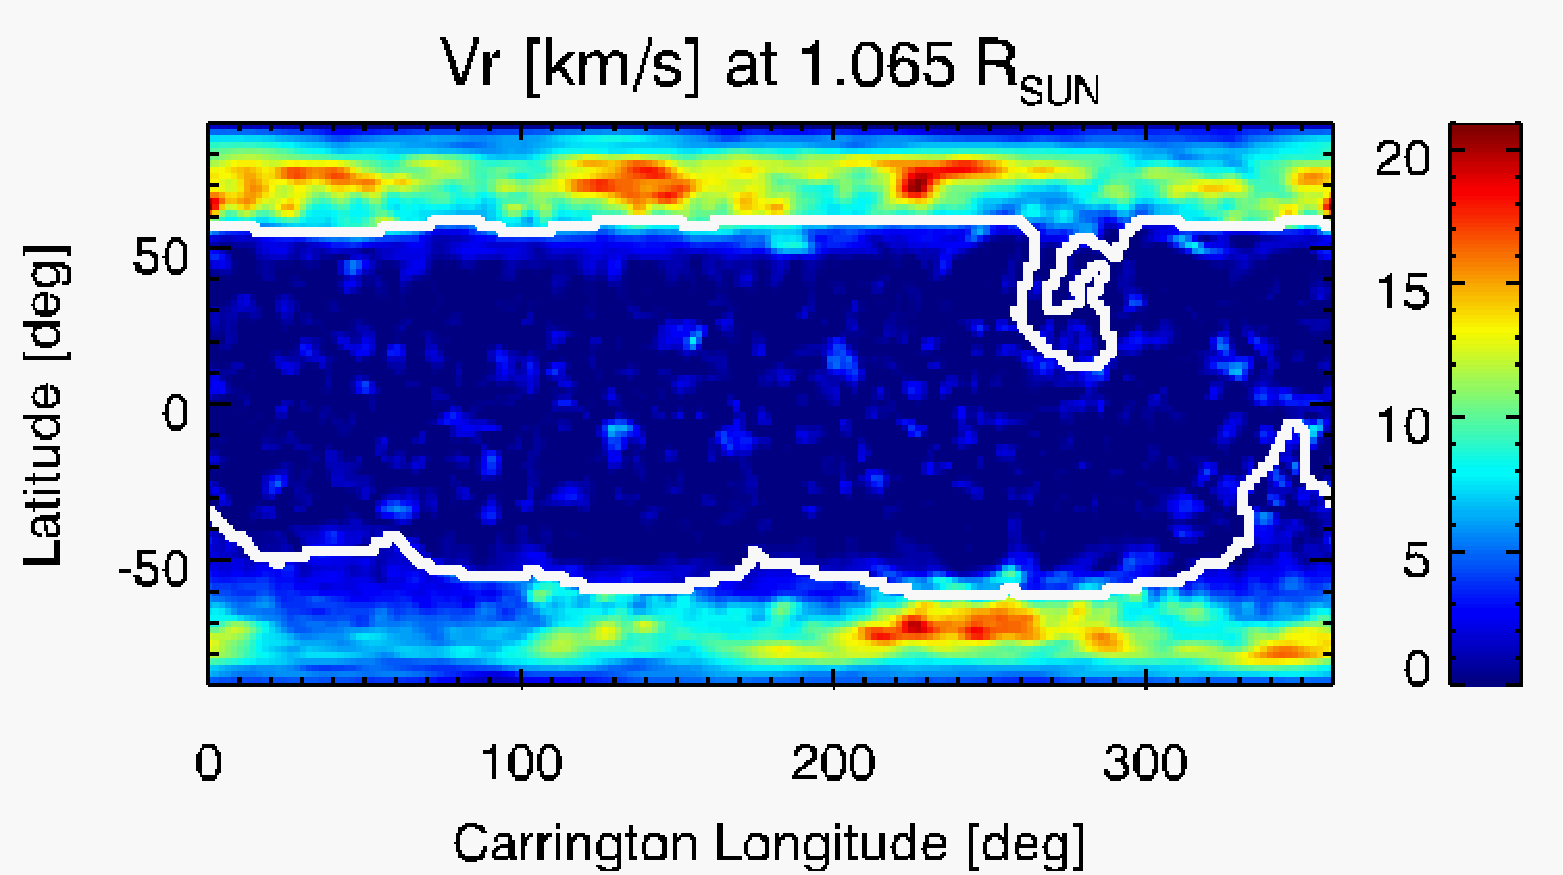
\includegraphics[width=0.65\textwidth]{new_figs/map_Vr_awsom_2223_realization10_extended_new_1065_Rsun_mapoc_awsom.pdf}\\
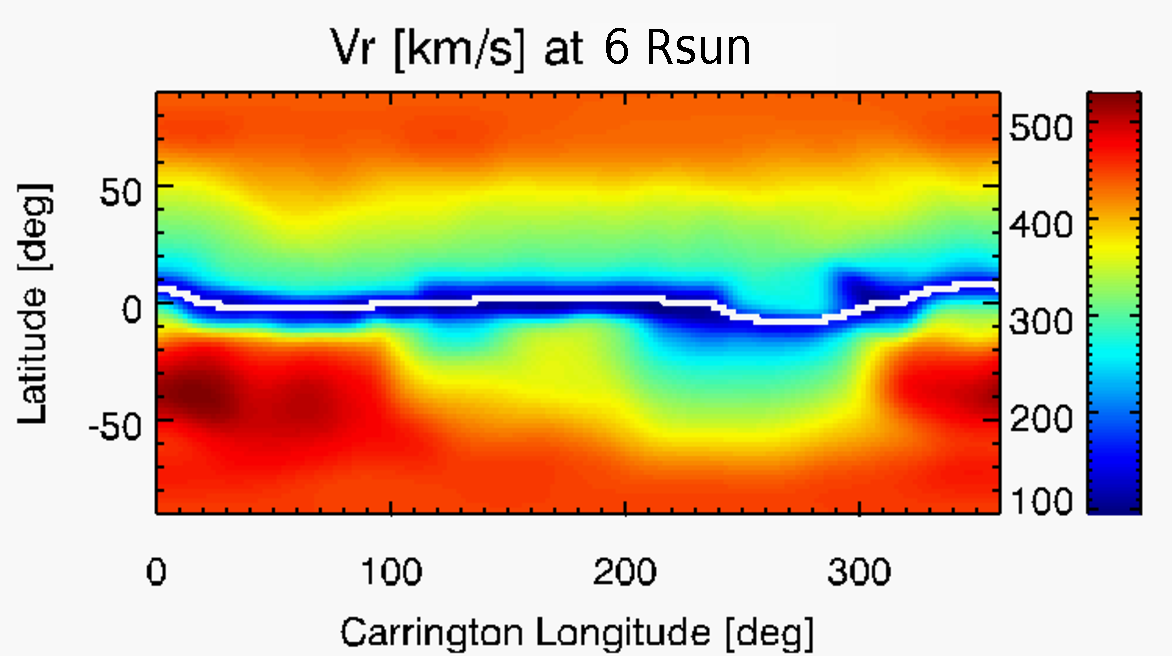
\includegraphics[width=0.65\textwidth]{new_figs/map_Vr_awsom_2223_realization10_extended_new_5945_Rsun_mapoc_awsom.pdf}
%map_Vr_awsom_2223_realization10_extended_new_5945_Rsun_2.pdf}
\end{center}
}

%---------------------------------
\begin{comment}
\frame{ 
\begin{columns}
\column{0.4\textwidth}
\begin{center}
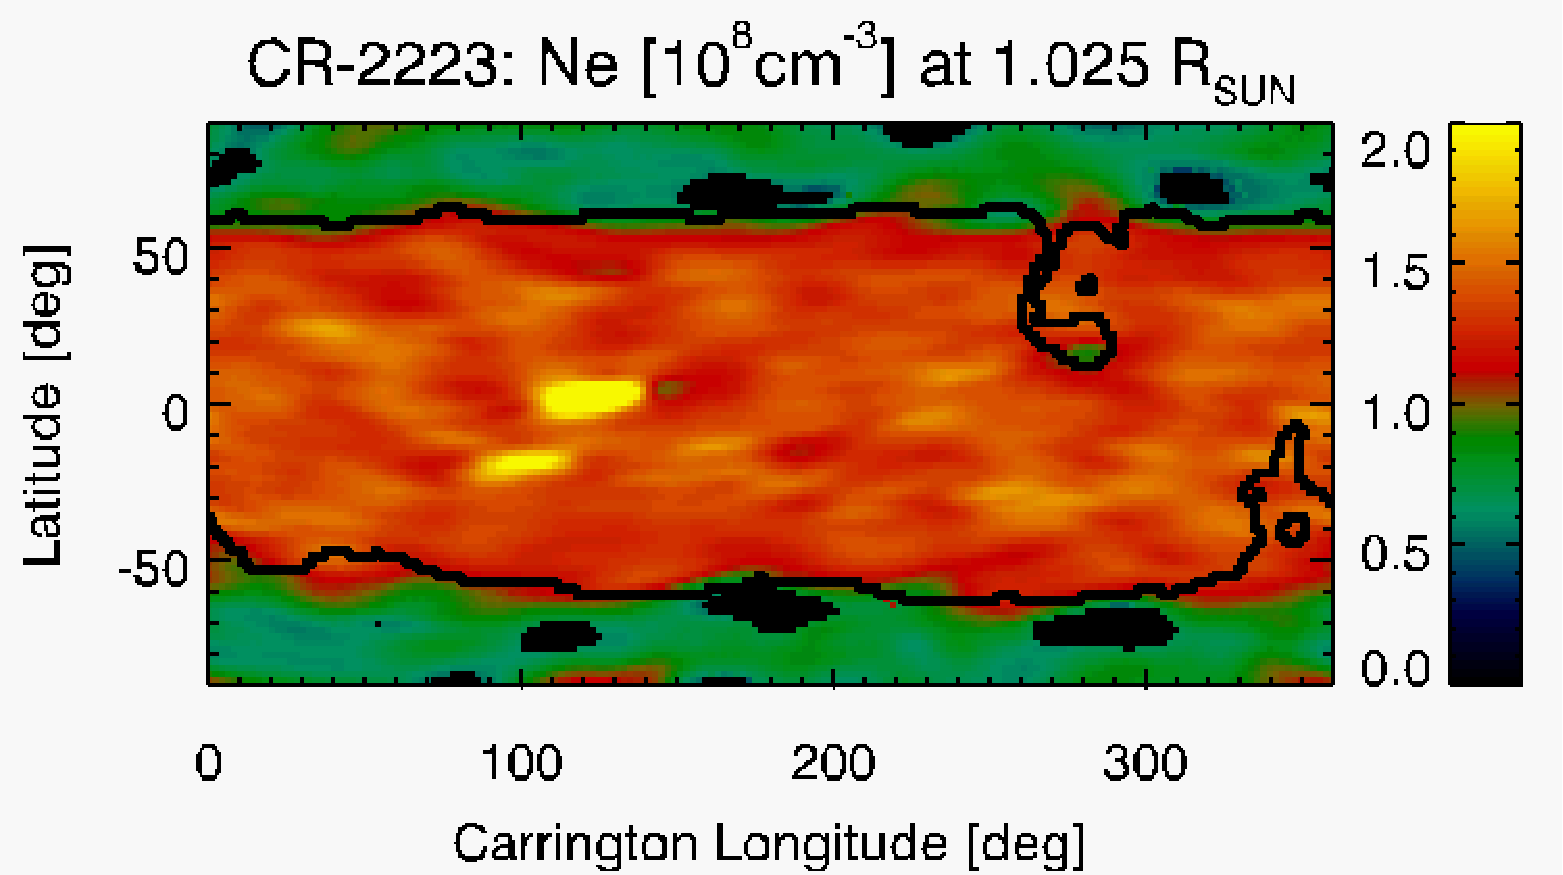
\includegraphics[width=0.99\textwidth]{new_figs/map_Ne_CR2223_DEMT-AIA_H1_L733_r3d_multistart_1025_Rsun_mapoc_awsom.pdf}\\
% \vspace{1.5cm}
%\raggedright
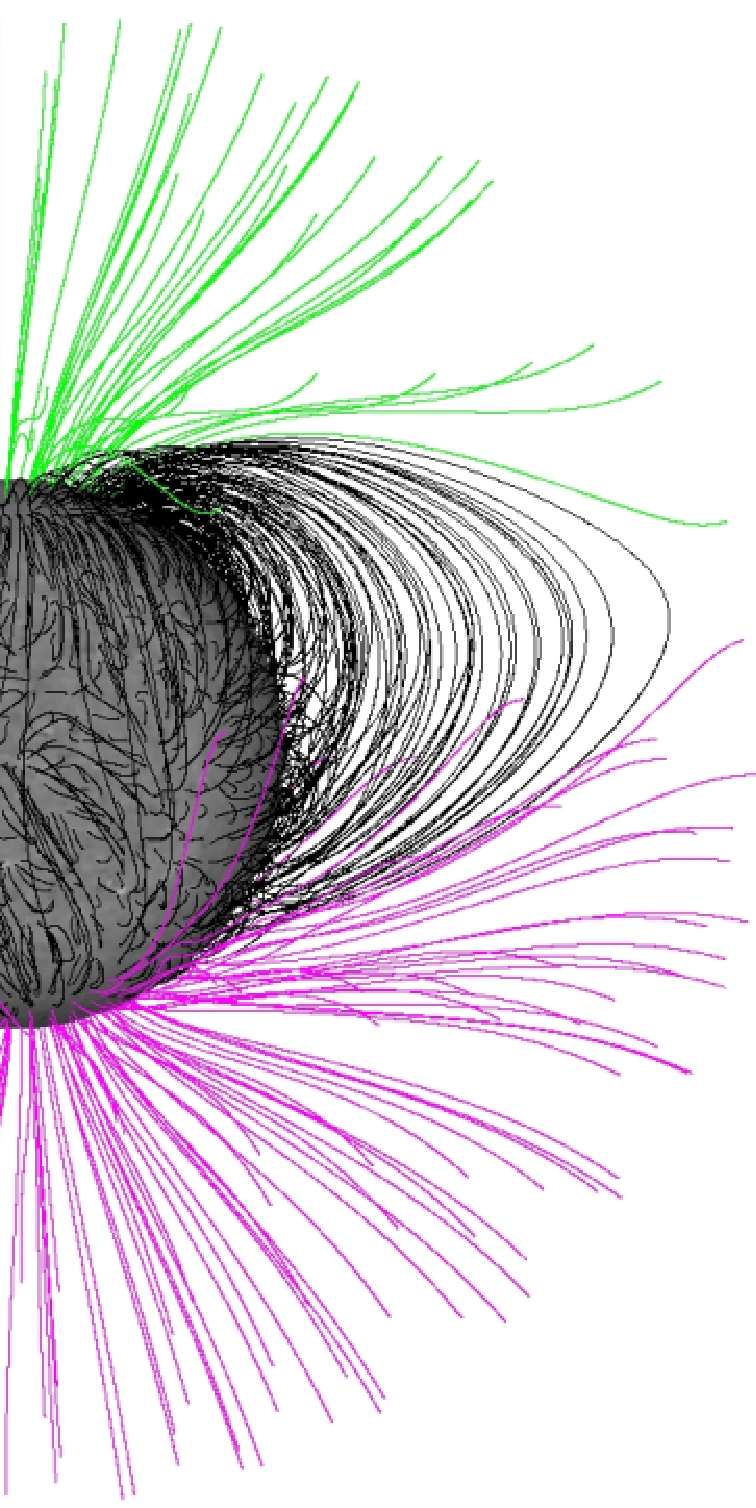
\includegraphics[width=0.3\textwidth]{new_figs/pfss_der.pdf}
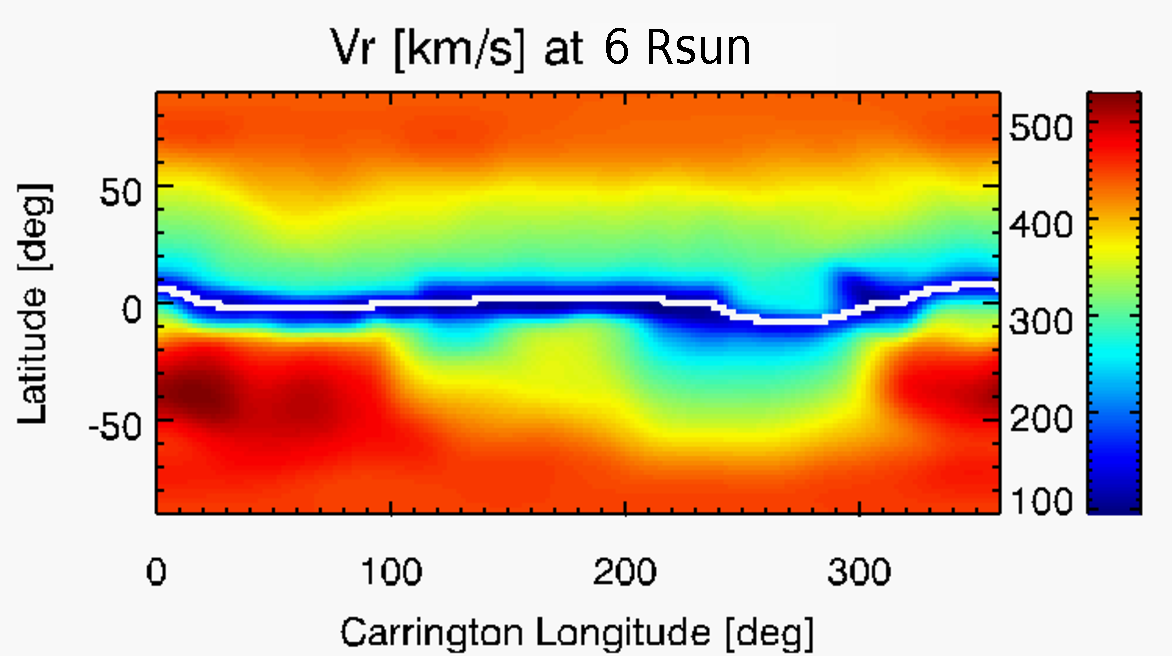
\includegraphics[width=0.99\textwidth]{new_figs/map_Vr_awsom_2223_realization10_extended_new_5945_Rsun_mapoc_awsom.pdf}
%map_Vr_awsom_2223_realization10_extended_new_5945_Rsun_2.pdf}
\end{center}
\column{0.6\textwidth}
\begin{center}
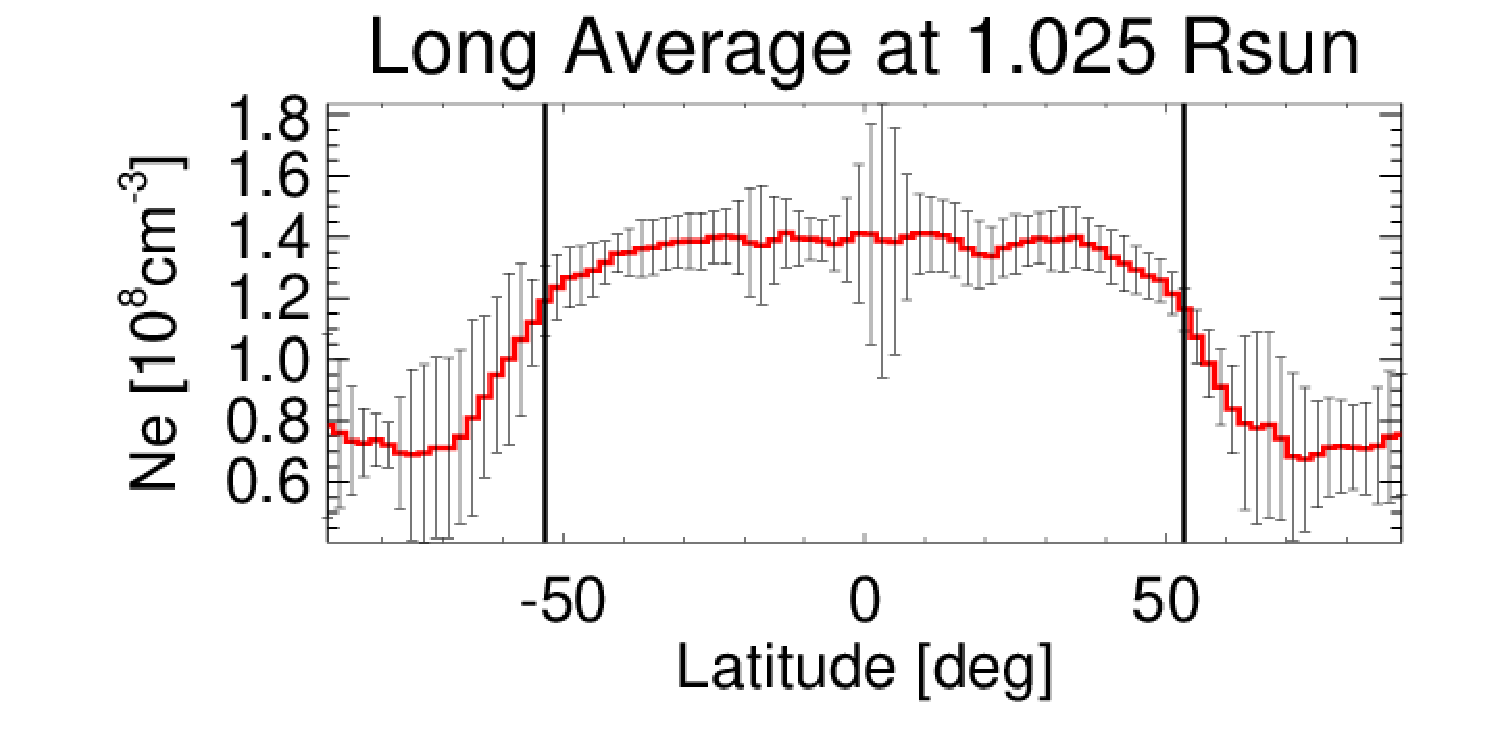
\includegraphics[width=0.99\textwidth]{new_figs/Perfil_Ne_demt_2223_basal_1025.pdf}\\
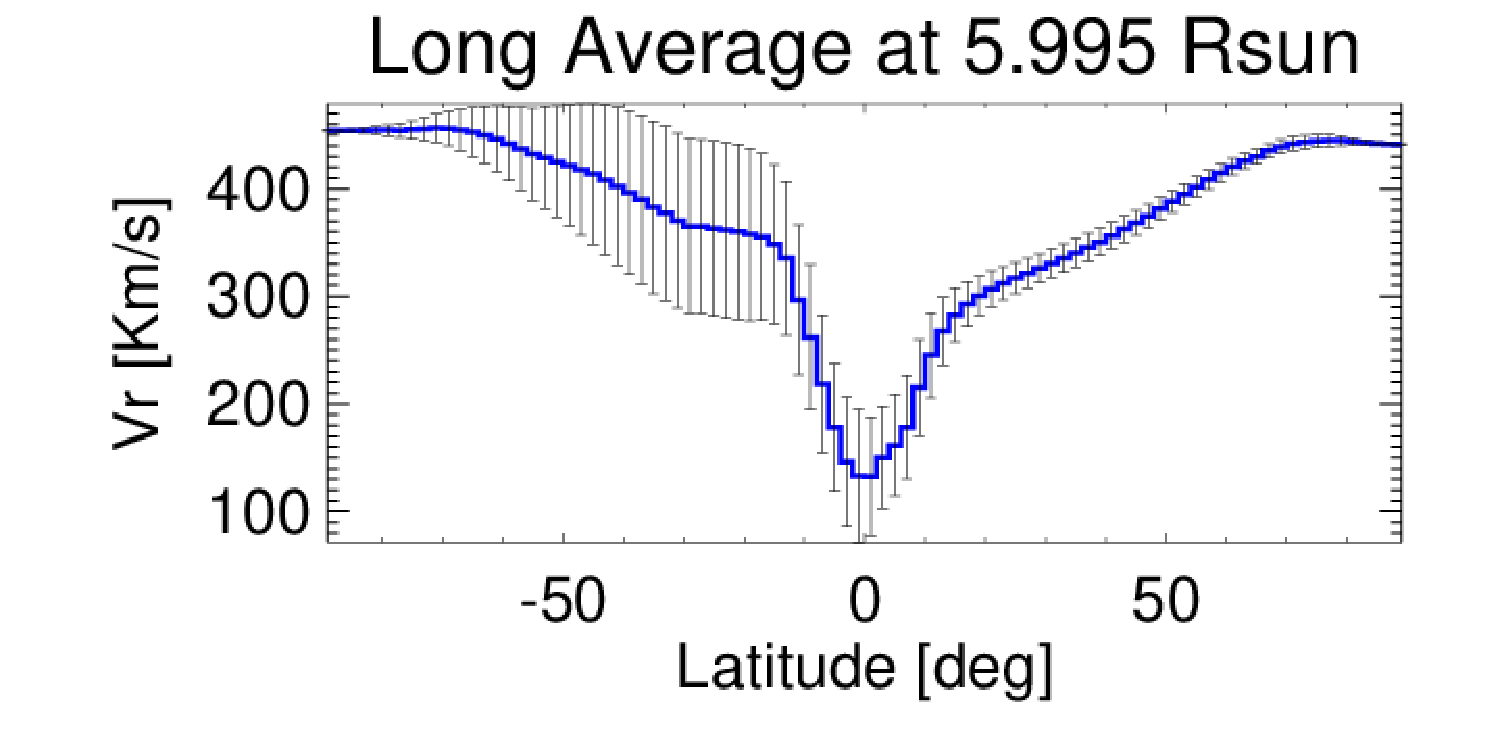
\includegraphics[width=0.99\textwidth]{new_figs/Perfil_Vr_awsom_2223_6rs_5995.pdf}\\
\end{center}

\end{columns}
}
\end{comment}
%---------------------------------
\frame{ 
\begin{center}
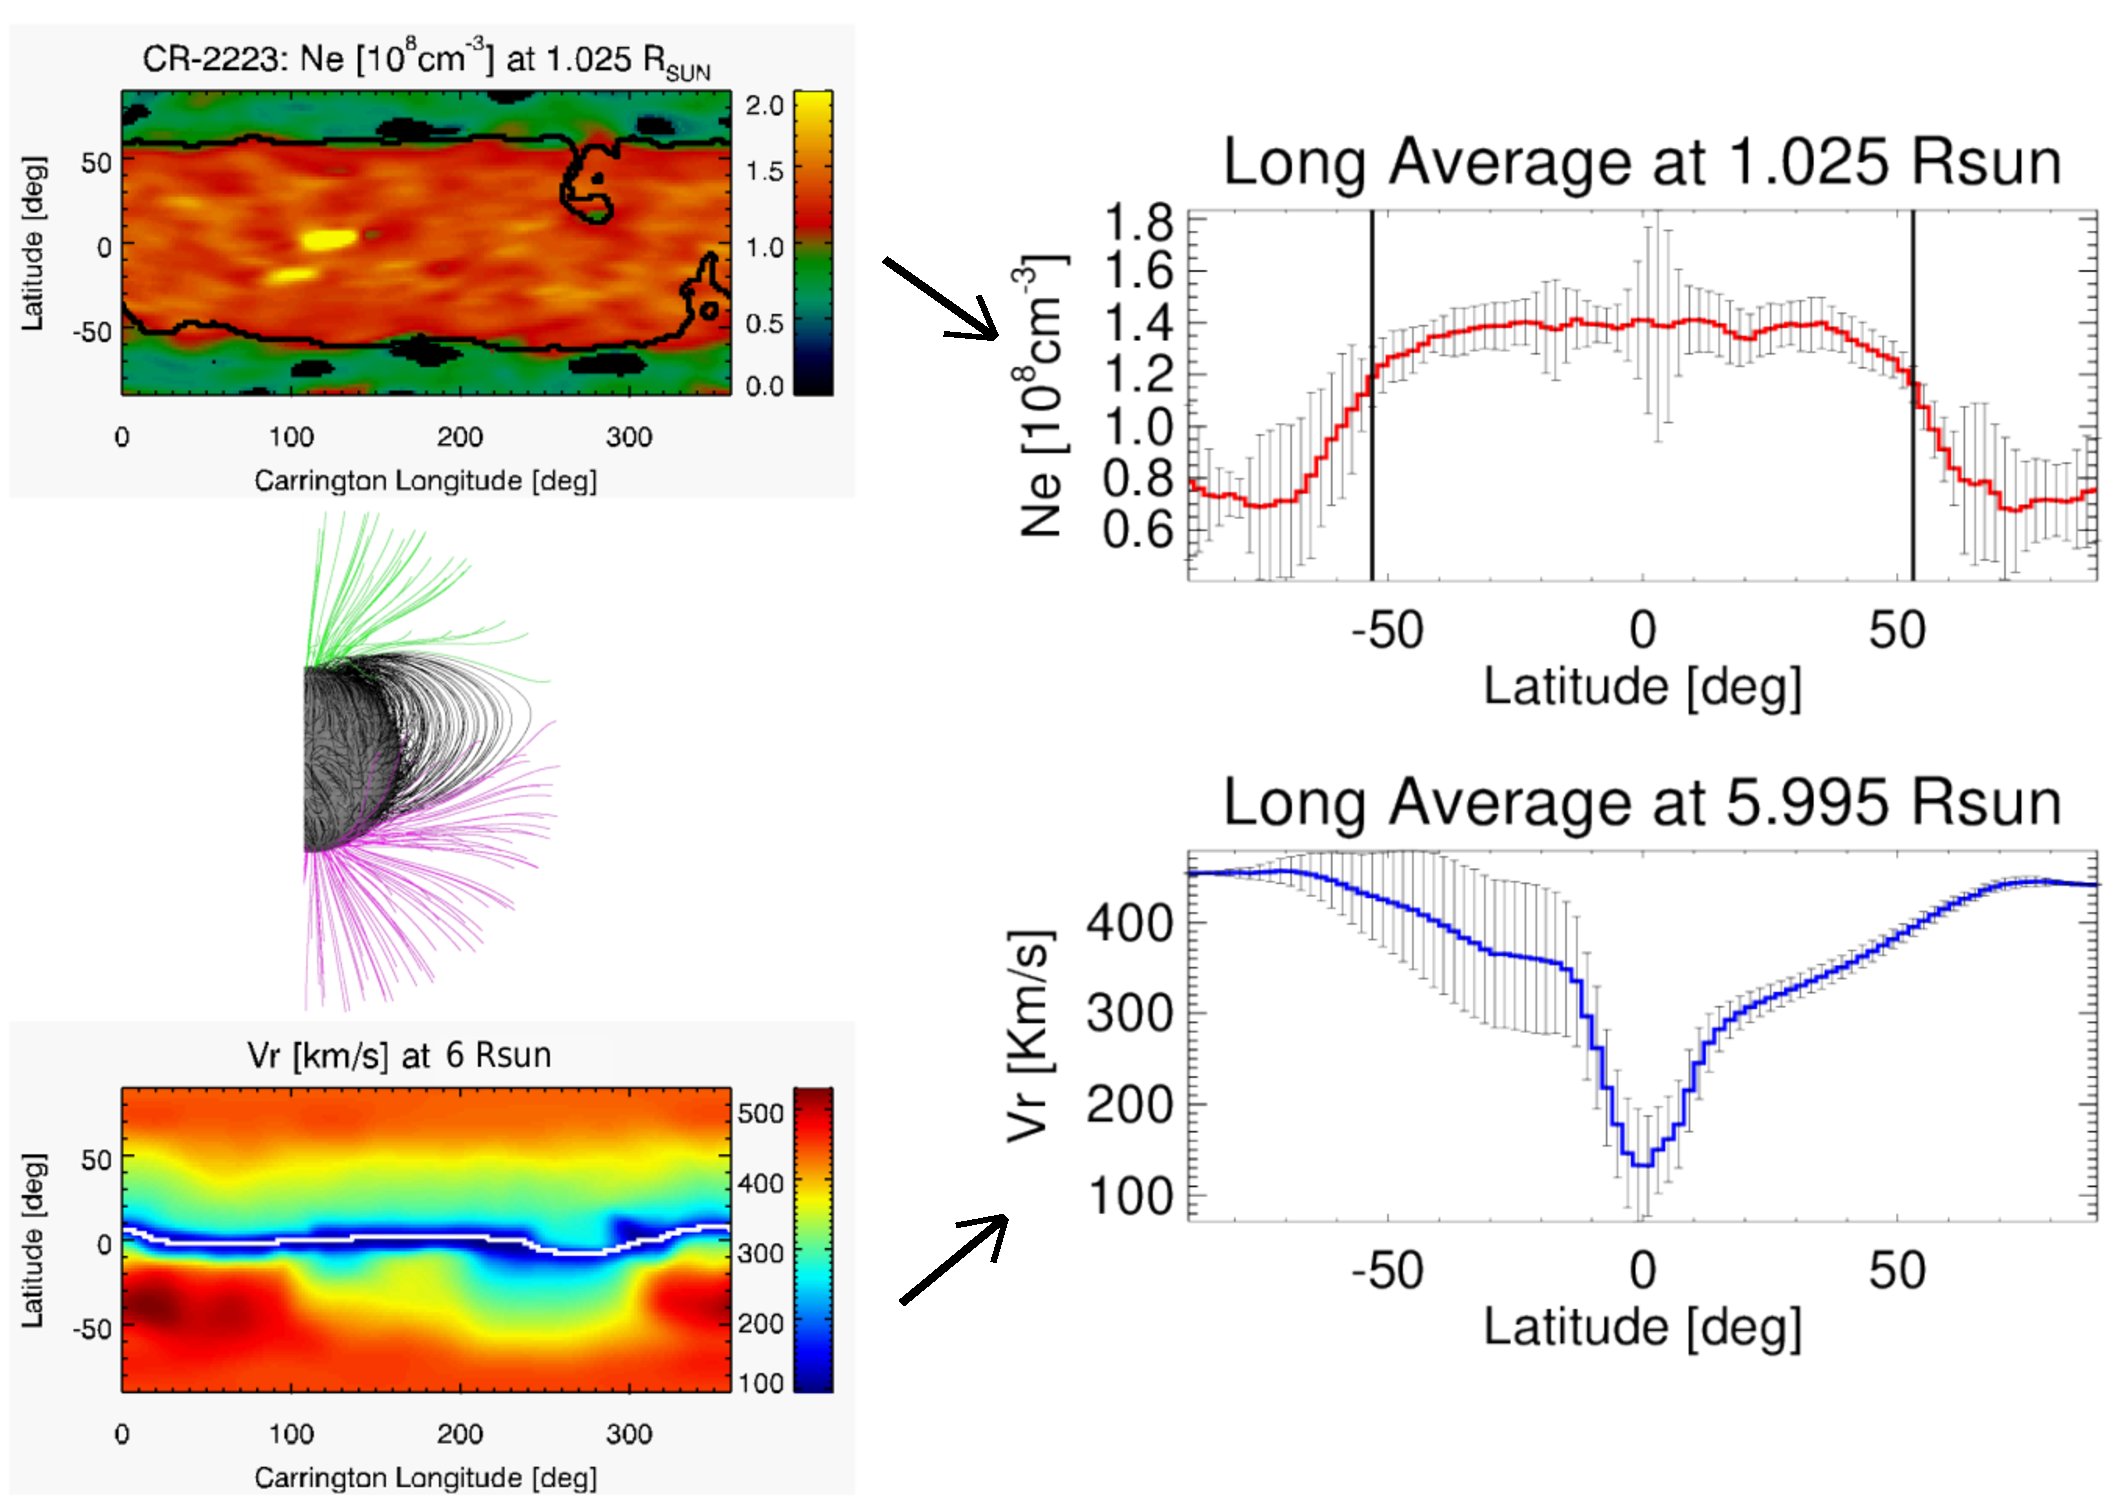
\includegraphics[width=0.9\textwidth]{new_figs/compost.pdf}\\
\end{center}
}
%---------------------------------

\frame{ 
\begin{center}
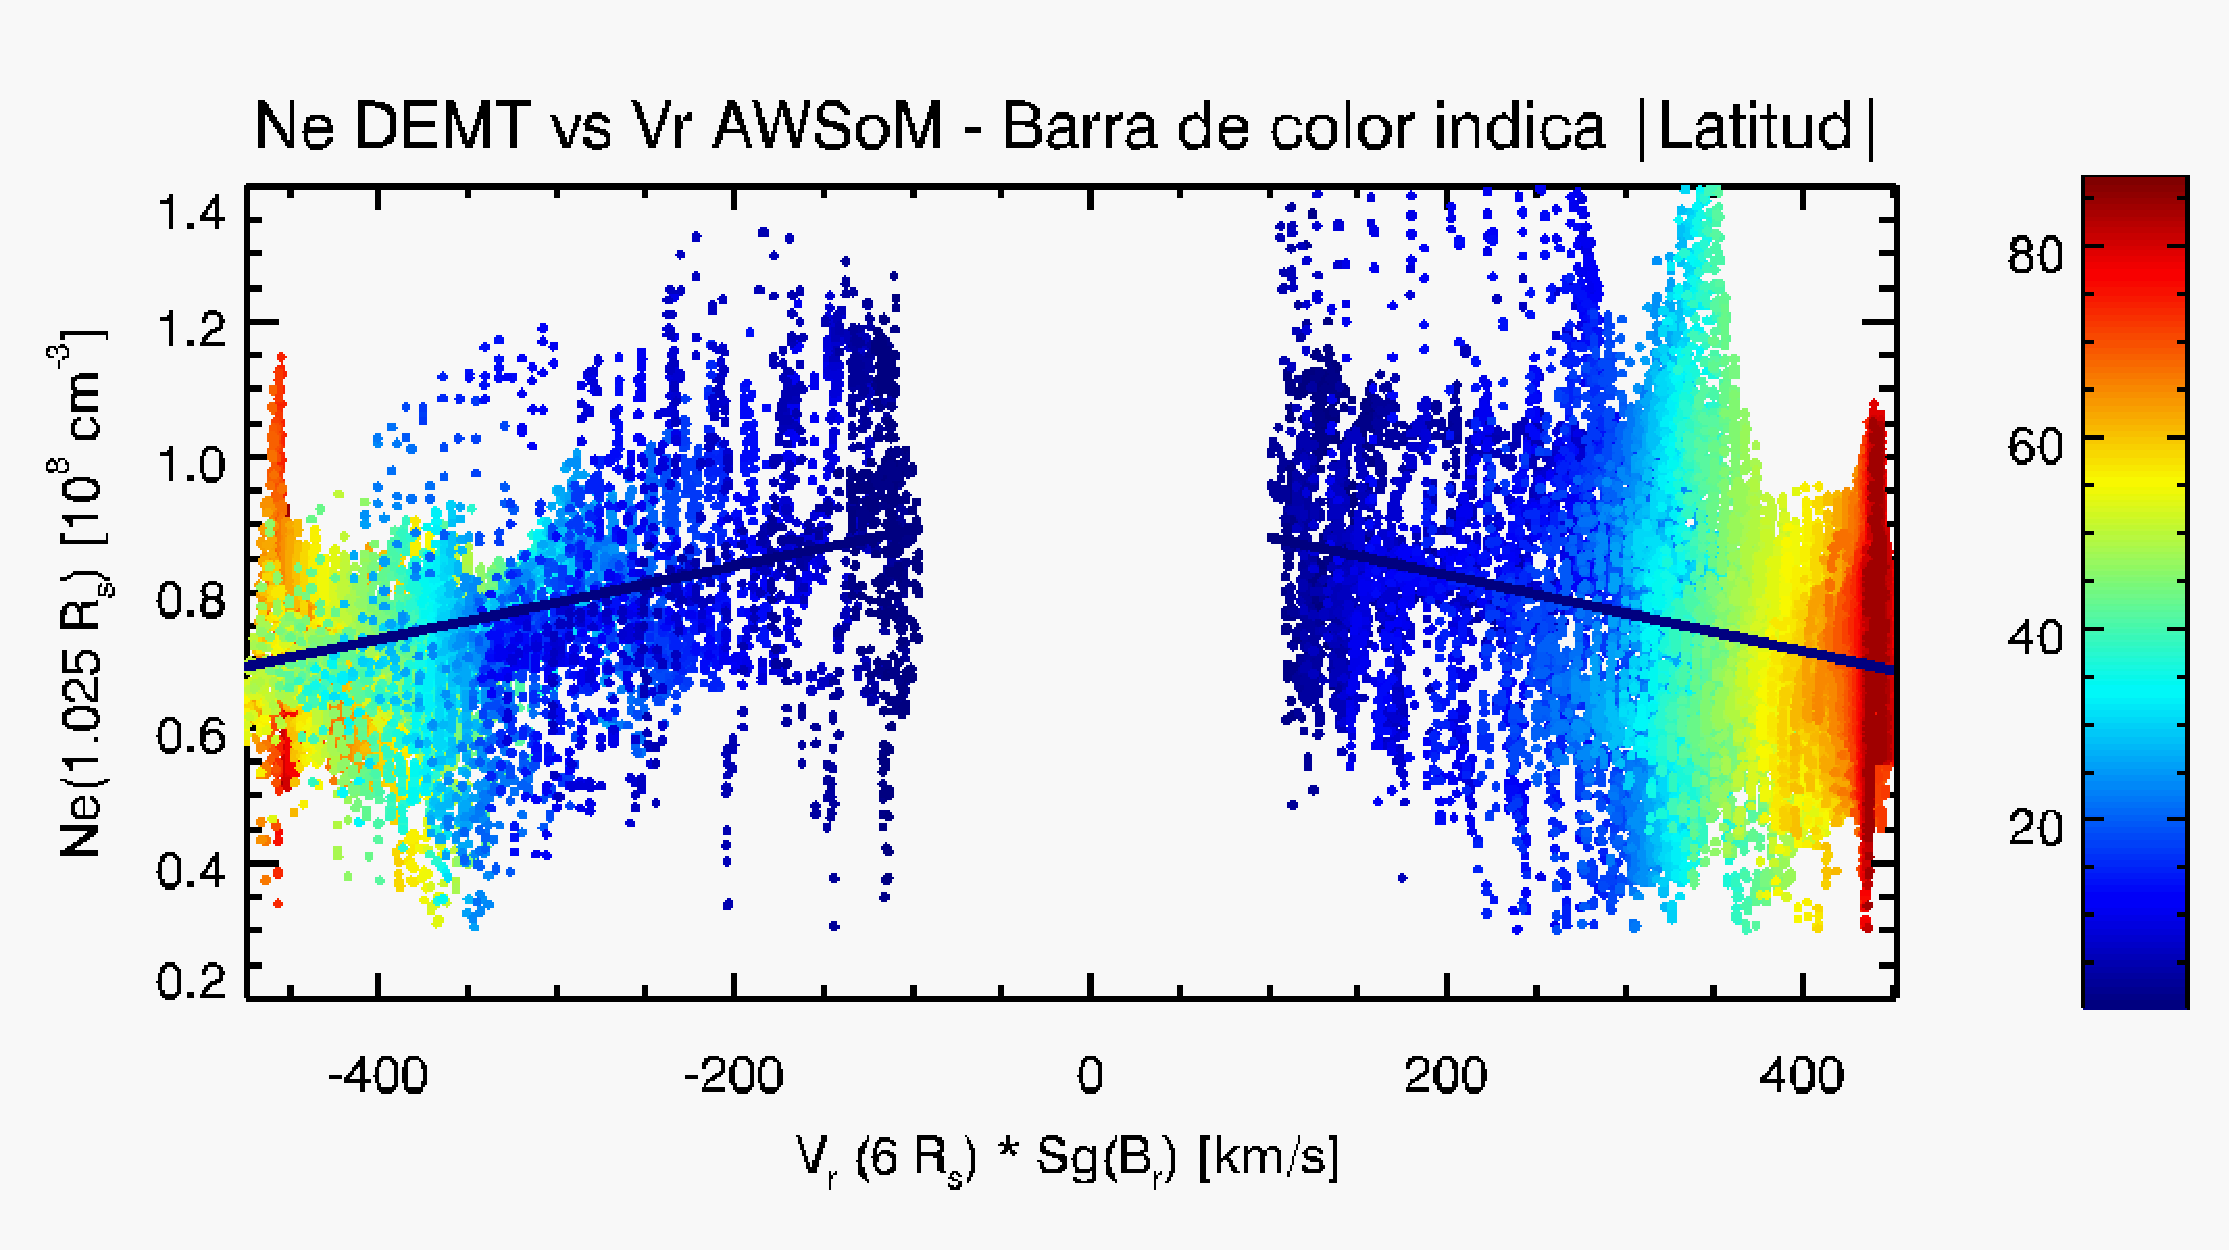
\includegraphics[width=0.99\textwidth]{new_figs/scatter_plot_nedemt_vs_vrxsignoBrCR2223_AWSoM_DEMT_ca_colbarlat.pdf}\\
\end{center}
\begin{itemize}
\item Determinamos tomograficamente y en forma cuantitativa, por primera vez,   propiedades basales de ambas componentes del viento solar
\end{itemize}
}
%--------------------------------------------------------------------------------

\frame{
\vspace{-0.05cm}
%\titulo{Trabajo futuro}
%\footnotesize
\Large{\azul{Comentarios finales}}
\normalsize{
\begin{itemize}
\item La Tomografía Solar Rotacional es actualmente la única técnica observacional que permite generar mapas 3D globales de Ne y Te (validar modelos MHD-3D).
%\item Mediante el trazado de los resultados correlacionamos las propiedades físicas derivadas por tomografía en la base coronal para las líneas magnéticas de las componentes rápida/lenta del viento solar del modelo MHD. Es el primer estudio de este tipo.
\item Trazando los resultados pudimos correlacionar las propiedades físicas en la base coronal obtenidas con la tomografia con las componentes rapida/lentas del viento solar dadas por el modelo MHD para cada línea magnéticamente abierta. 
%\item Determinamos tomograficamente y en forma cuantitativa 3D, por primera vez,   propiedades basales del viento solar rápido/lento.

\end{itemize}
}
\vspace{1cm}
\Large{\azul{Trabajo futuro}}
\normalsize{
\begin{itemize}
\item Nuevos modelados MHD utilizando magnetogramas co-centrados temporalmente con imágenes EUV, para CR-2219 y CR-2223.\\
\item Agregado de propiedades terminales.
\item Incorporación de tomografía utilizando imágenes de Lasco-C2 (LAM) para cubrir el rango $2.5-6.0$ {R$_{SUN}$}.
\end{itemize}
}

%\item Por debajo de $r \sim 1.05 \ {\rm R_{SUN}}$ el modelo AWSoM no es capaz de modelar la baja corona (region de transicion extendida). 
%\item Sobre $r \sim 1.05 \ {\rm R_{SUN}}$ en Streamer y Agujero Coronal: $T_e$ y $N_e$ en acuerdo dentro del $\sim 30 \%$.
%\item Realizar una rotación mas cercana al mínimo $\rightarrow$ Whole Heliosphere and Planetary Interactions (WHPI)
%\item Implementación de Tomografía Multi Instrumental (EUV: EUVI, AIA; Luz Blanca: K-cor, Lasco-C2;  Coronal Multichannel Polarimeter (CoMP). 


}




\end{document}

% Slides extra
